\chapter{Spectral ViT Model Performance}
\label{chap:results}

\section{Spectral ViT V1: A suitable replacement}\label{sec:v1_results}
The Spectral ViT's performance was evaluated on the test set of 12888 validation spectra.
These spectra were not used in the training, nor the test set of the model. The resulting 
ROC curve and confusion matrix are shown in Figure~\ref{fig:v1_qual}. The ROC curve 
shows the model is capable of differentiating between SNe and non-SNe with an AUC of 0.99.
However, differentiating between the different types of SNe is more difficult, as the
confusion matrix indicates. 
\begin{figure}
    \centering
    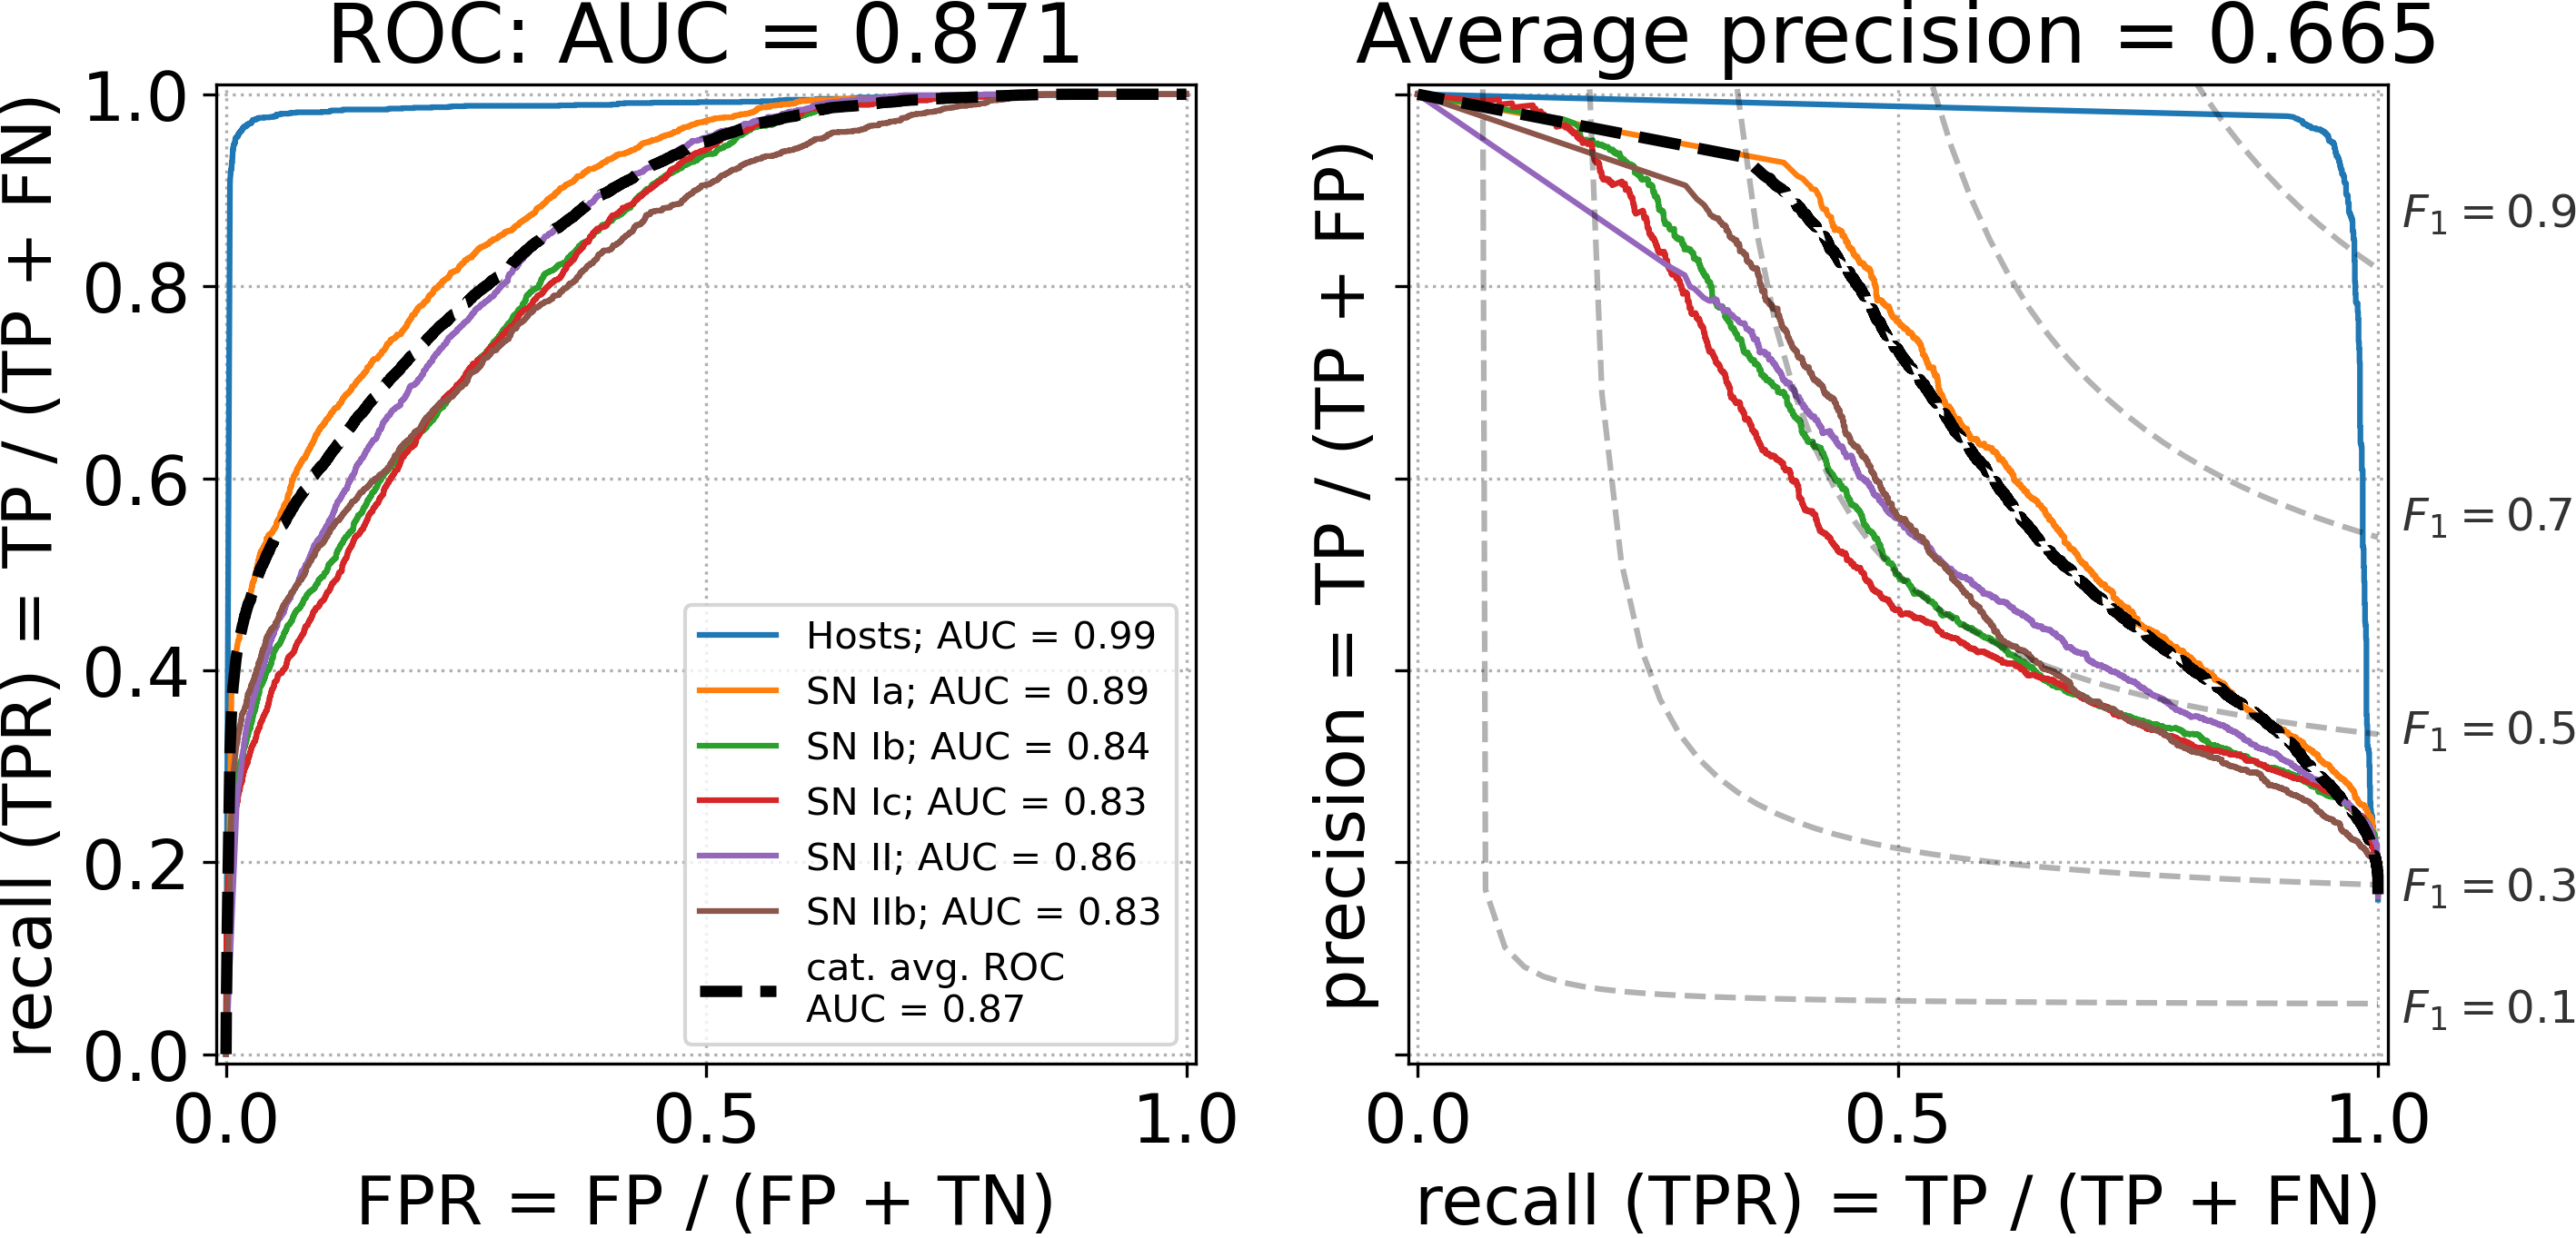
\includegraphics[height=4.3cm]{figures/v1_real/vit_model_V1_original_redorocfulle_e31.png}
    \quad
    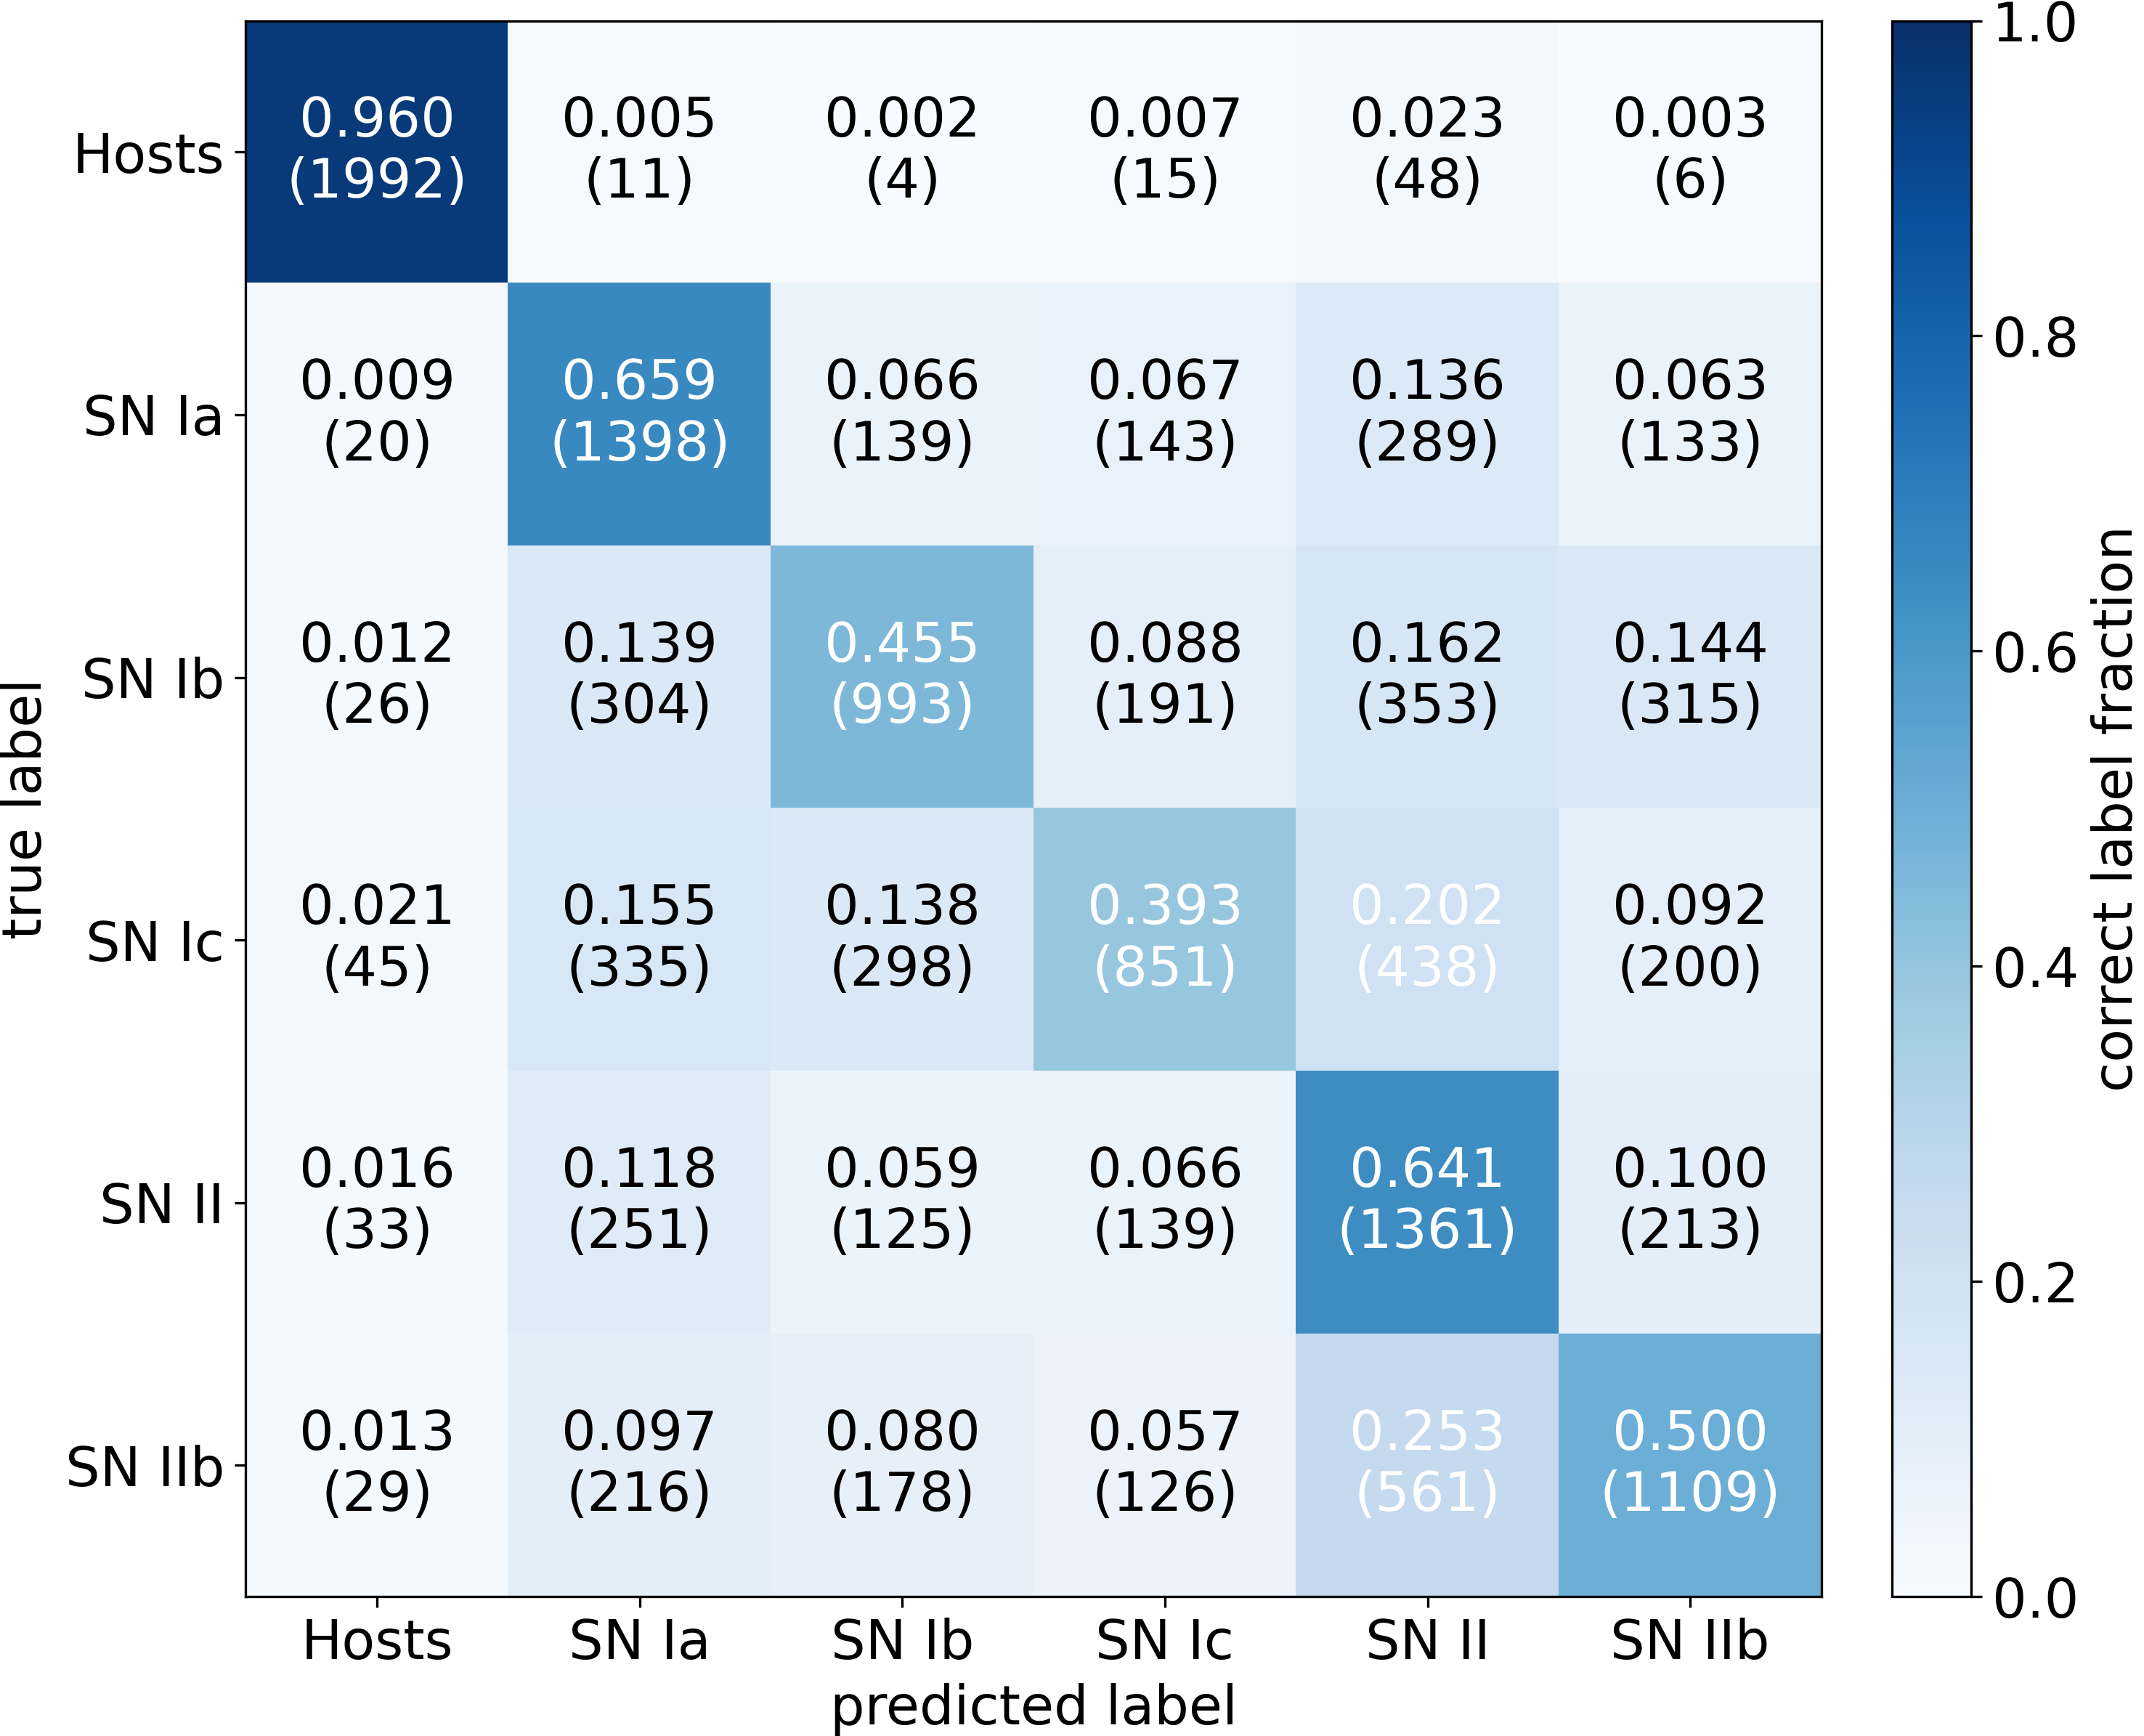
\includegraphics[height=4.3cm]{figures/v1_real/vit_model_V1_original_redocmfull_e31.png}
    \caption[Spectral ViT V1 Diagnostics]{Spectral ViT V1 Diagnostics: ROC Curve (left) and Confusion Matrix (right)\label{fig:v1_qual}}
\end{figure}

In contrast to the CNN previously used by \textcite{Sepeku2022}, the Spectral ViT V1 
was more sure of its predictions, as indicated by Figure~\ref{fig:v1_max}. By filtering 
out predictions with a maximum value less than 99\%, the model's average precision 
was increased from 0.665 to 0.783 (Figure~\ref{fig:v1_99_qual}). This cut included 
63.4\% of the original predictions. Further increasing this cut to 99.9999\% reduced 
the sample size to 5156 (40\% of the original validation size), but further increased the 
average precision to 86.2\%, as shown in Figure~\ref{fig:v1_999999_qual}.  
\begin{figure}[t]
    \centering
    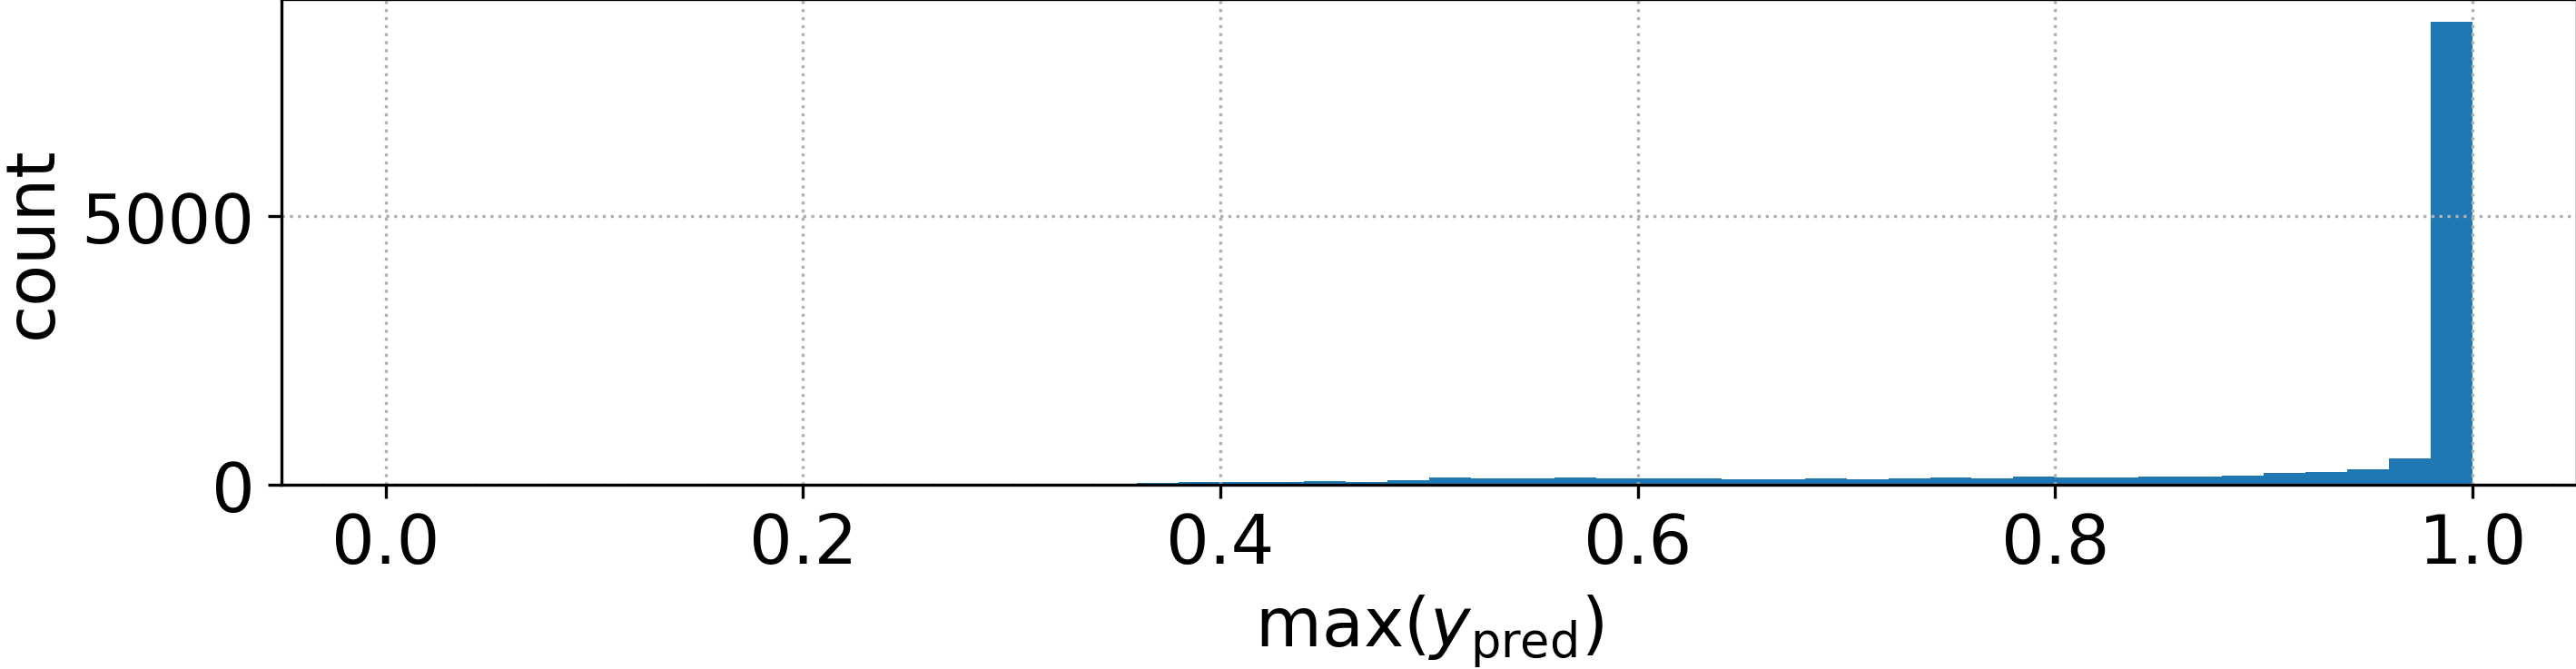
\includegraphics[width=0.8\textwidth]{figures/v1_real/vit_model_V1_original_redomax_ypred_binary_31.png}
    \caption[Spectral ViT V1 Confidence]{Max value of the output vector from the Spectral ViT V1.\label{fig:v1_max}}
\end{figure}

\begin{figure}[b]
    \centering
    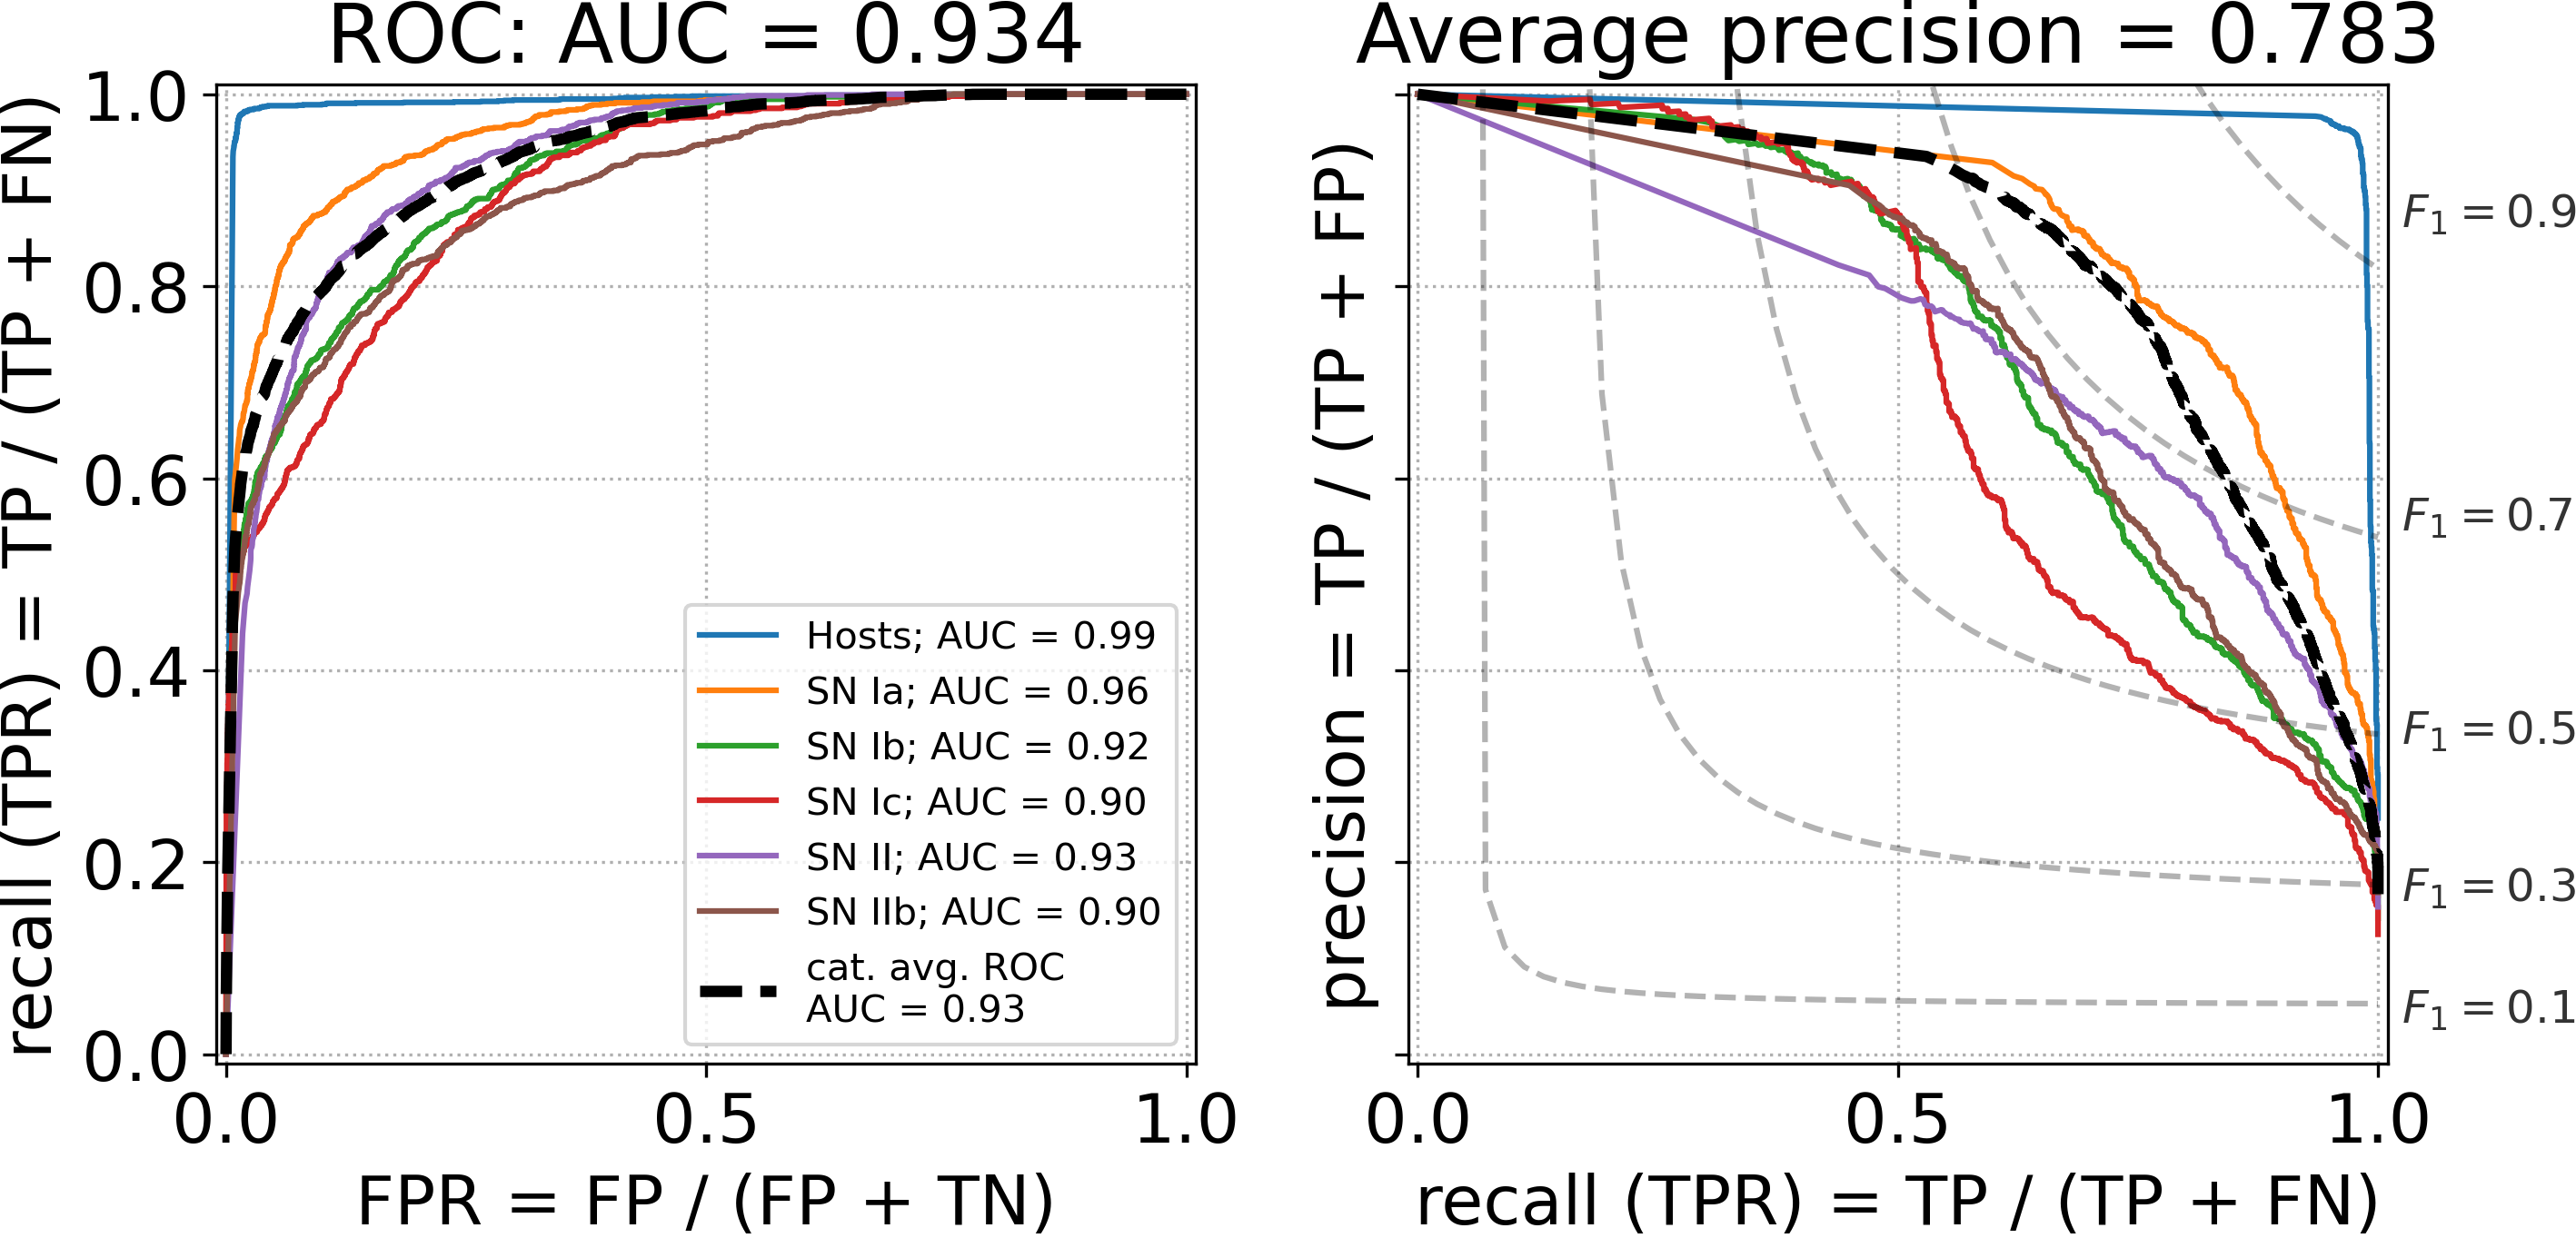
\includegraphics[height=4.3cm]{figures/v1_real/vit_model_V1_original_redoroc99_e31.png}
    \quad
    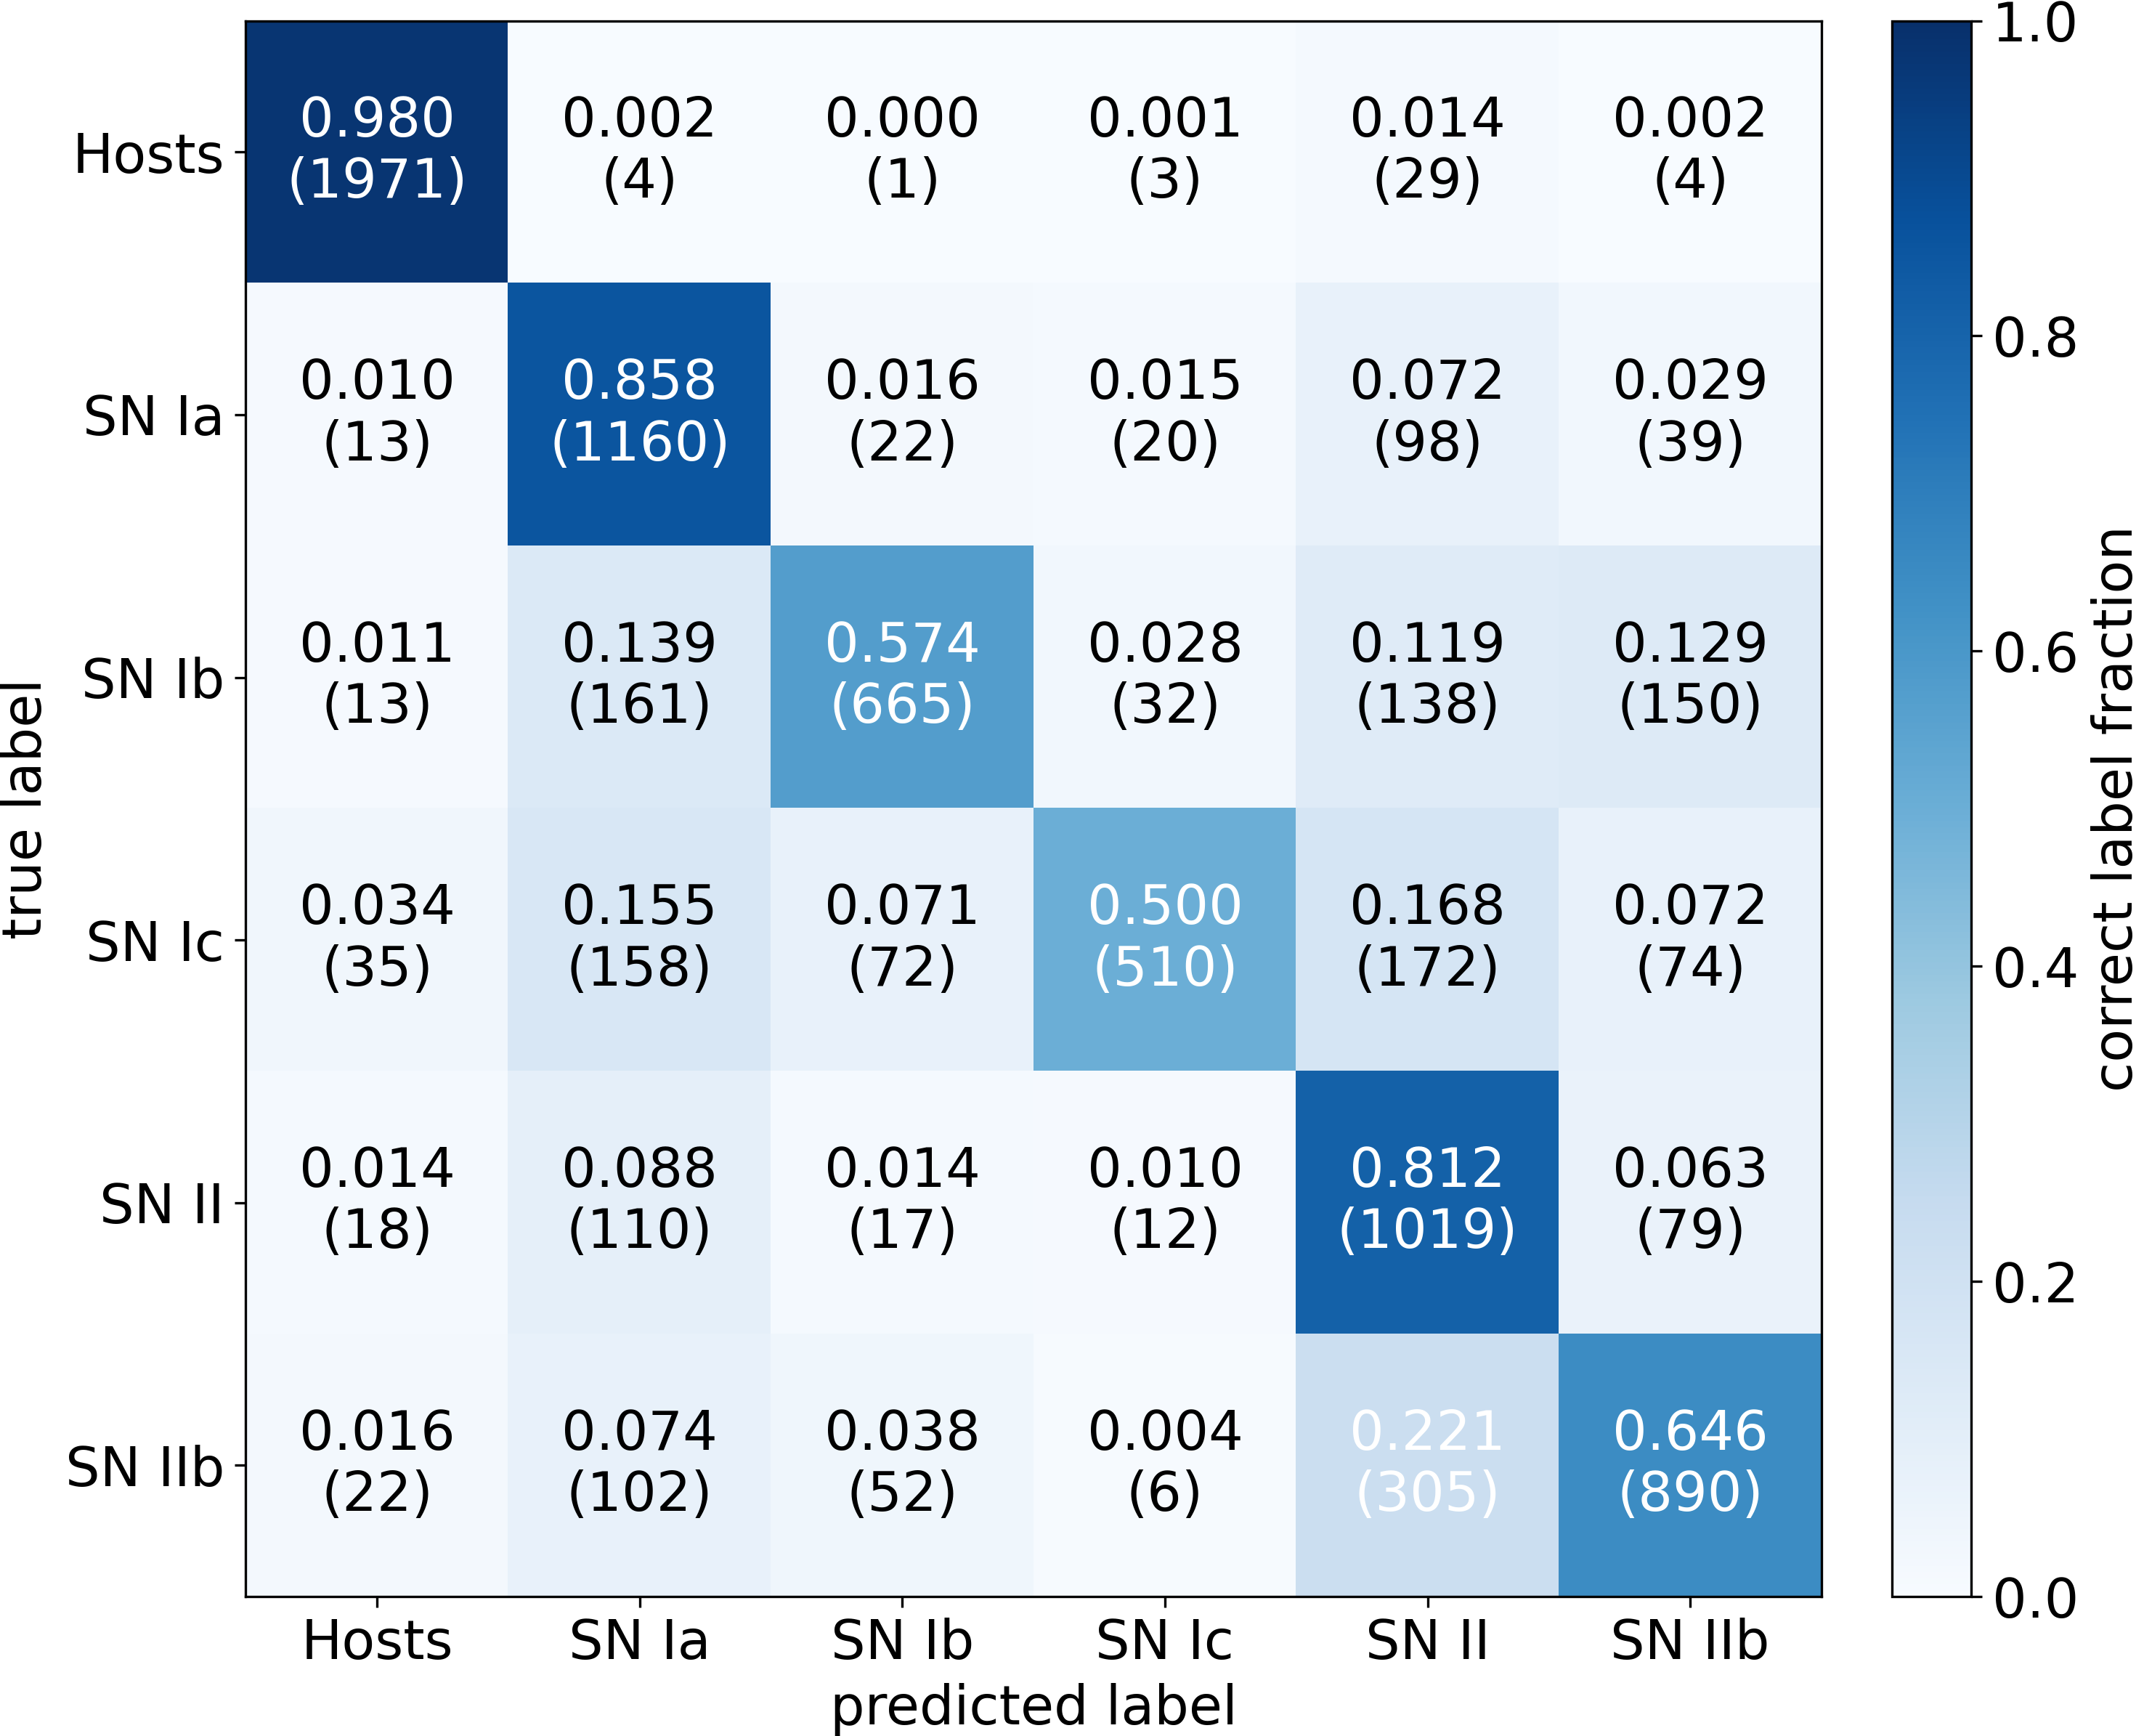
\includegraphics[height=4.3cm]{figures/v1_real/vit_model_V1_original_redocm99_e31.png}
    \caption[Spectral ViT V1 Diagnostics: 99\% Cut]{Spectral ViT V1 Diagnostics: ROC Curve (left) and Confusion Matrix (right) with a 99\% confidence
    cut \label{fig:v1_99_qual}}
\end{figure}

While the accuracy score didn't increase significantly with the second confidence cut, 
the important metric is the number of positive predictions made. All AUC scores 
are above 0.95, and the number of found targets is significantly higher than the 
CNN previously used. For example, Figure~\ref{fig:v1_999999_qual} correctly 
classifies 4705 targets, while Figure~\ref{fig:cnn_qual2} only correctly classifies 
3742 targets under a less strict confidence cut. This is a 26\% increase in the
number of correctly classified targets not excluded by the confidence cut.

\begin{figure}
    \centering
    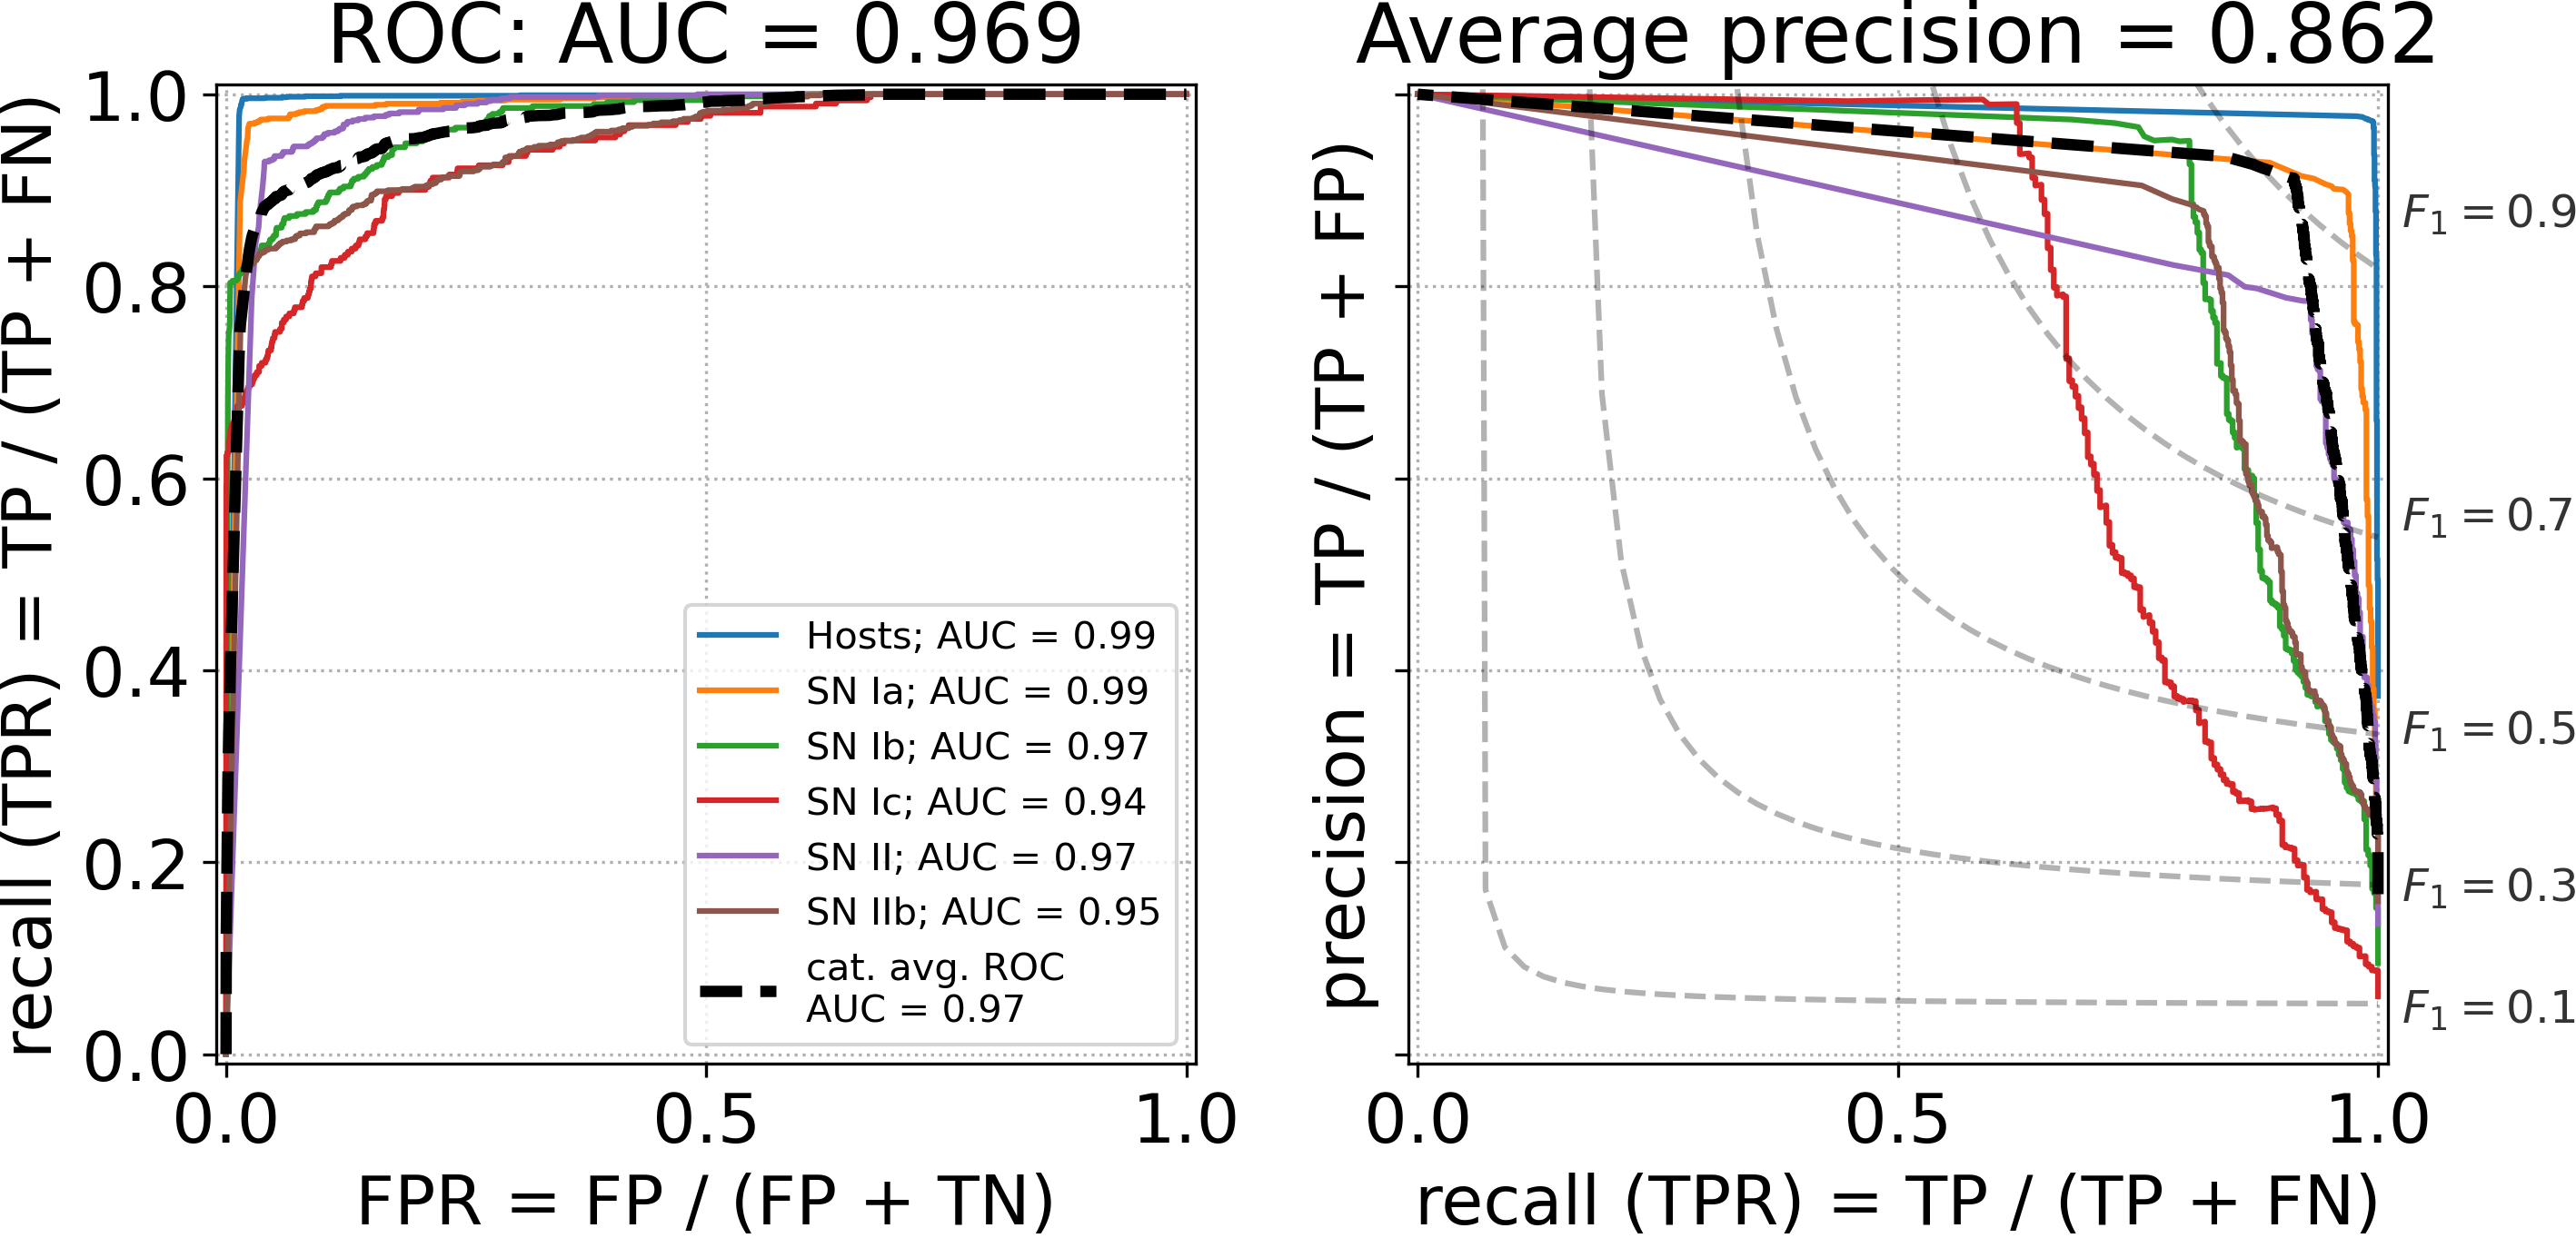
\includegraphics[height=4.3cm]{figures/v1_real/vit_model_V1_original_redoroc999999_e31.png}
    \quad
    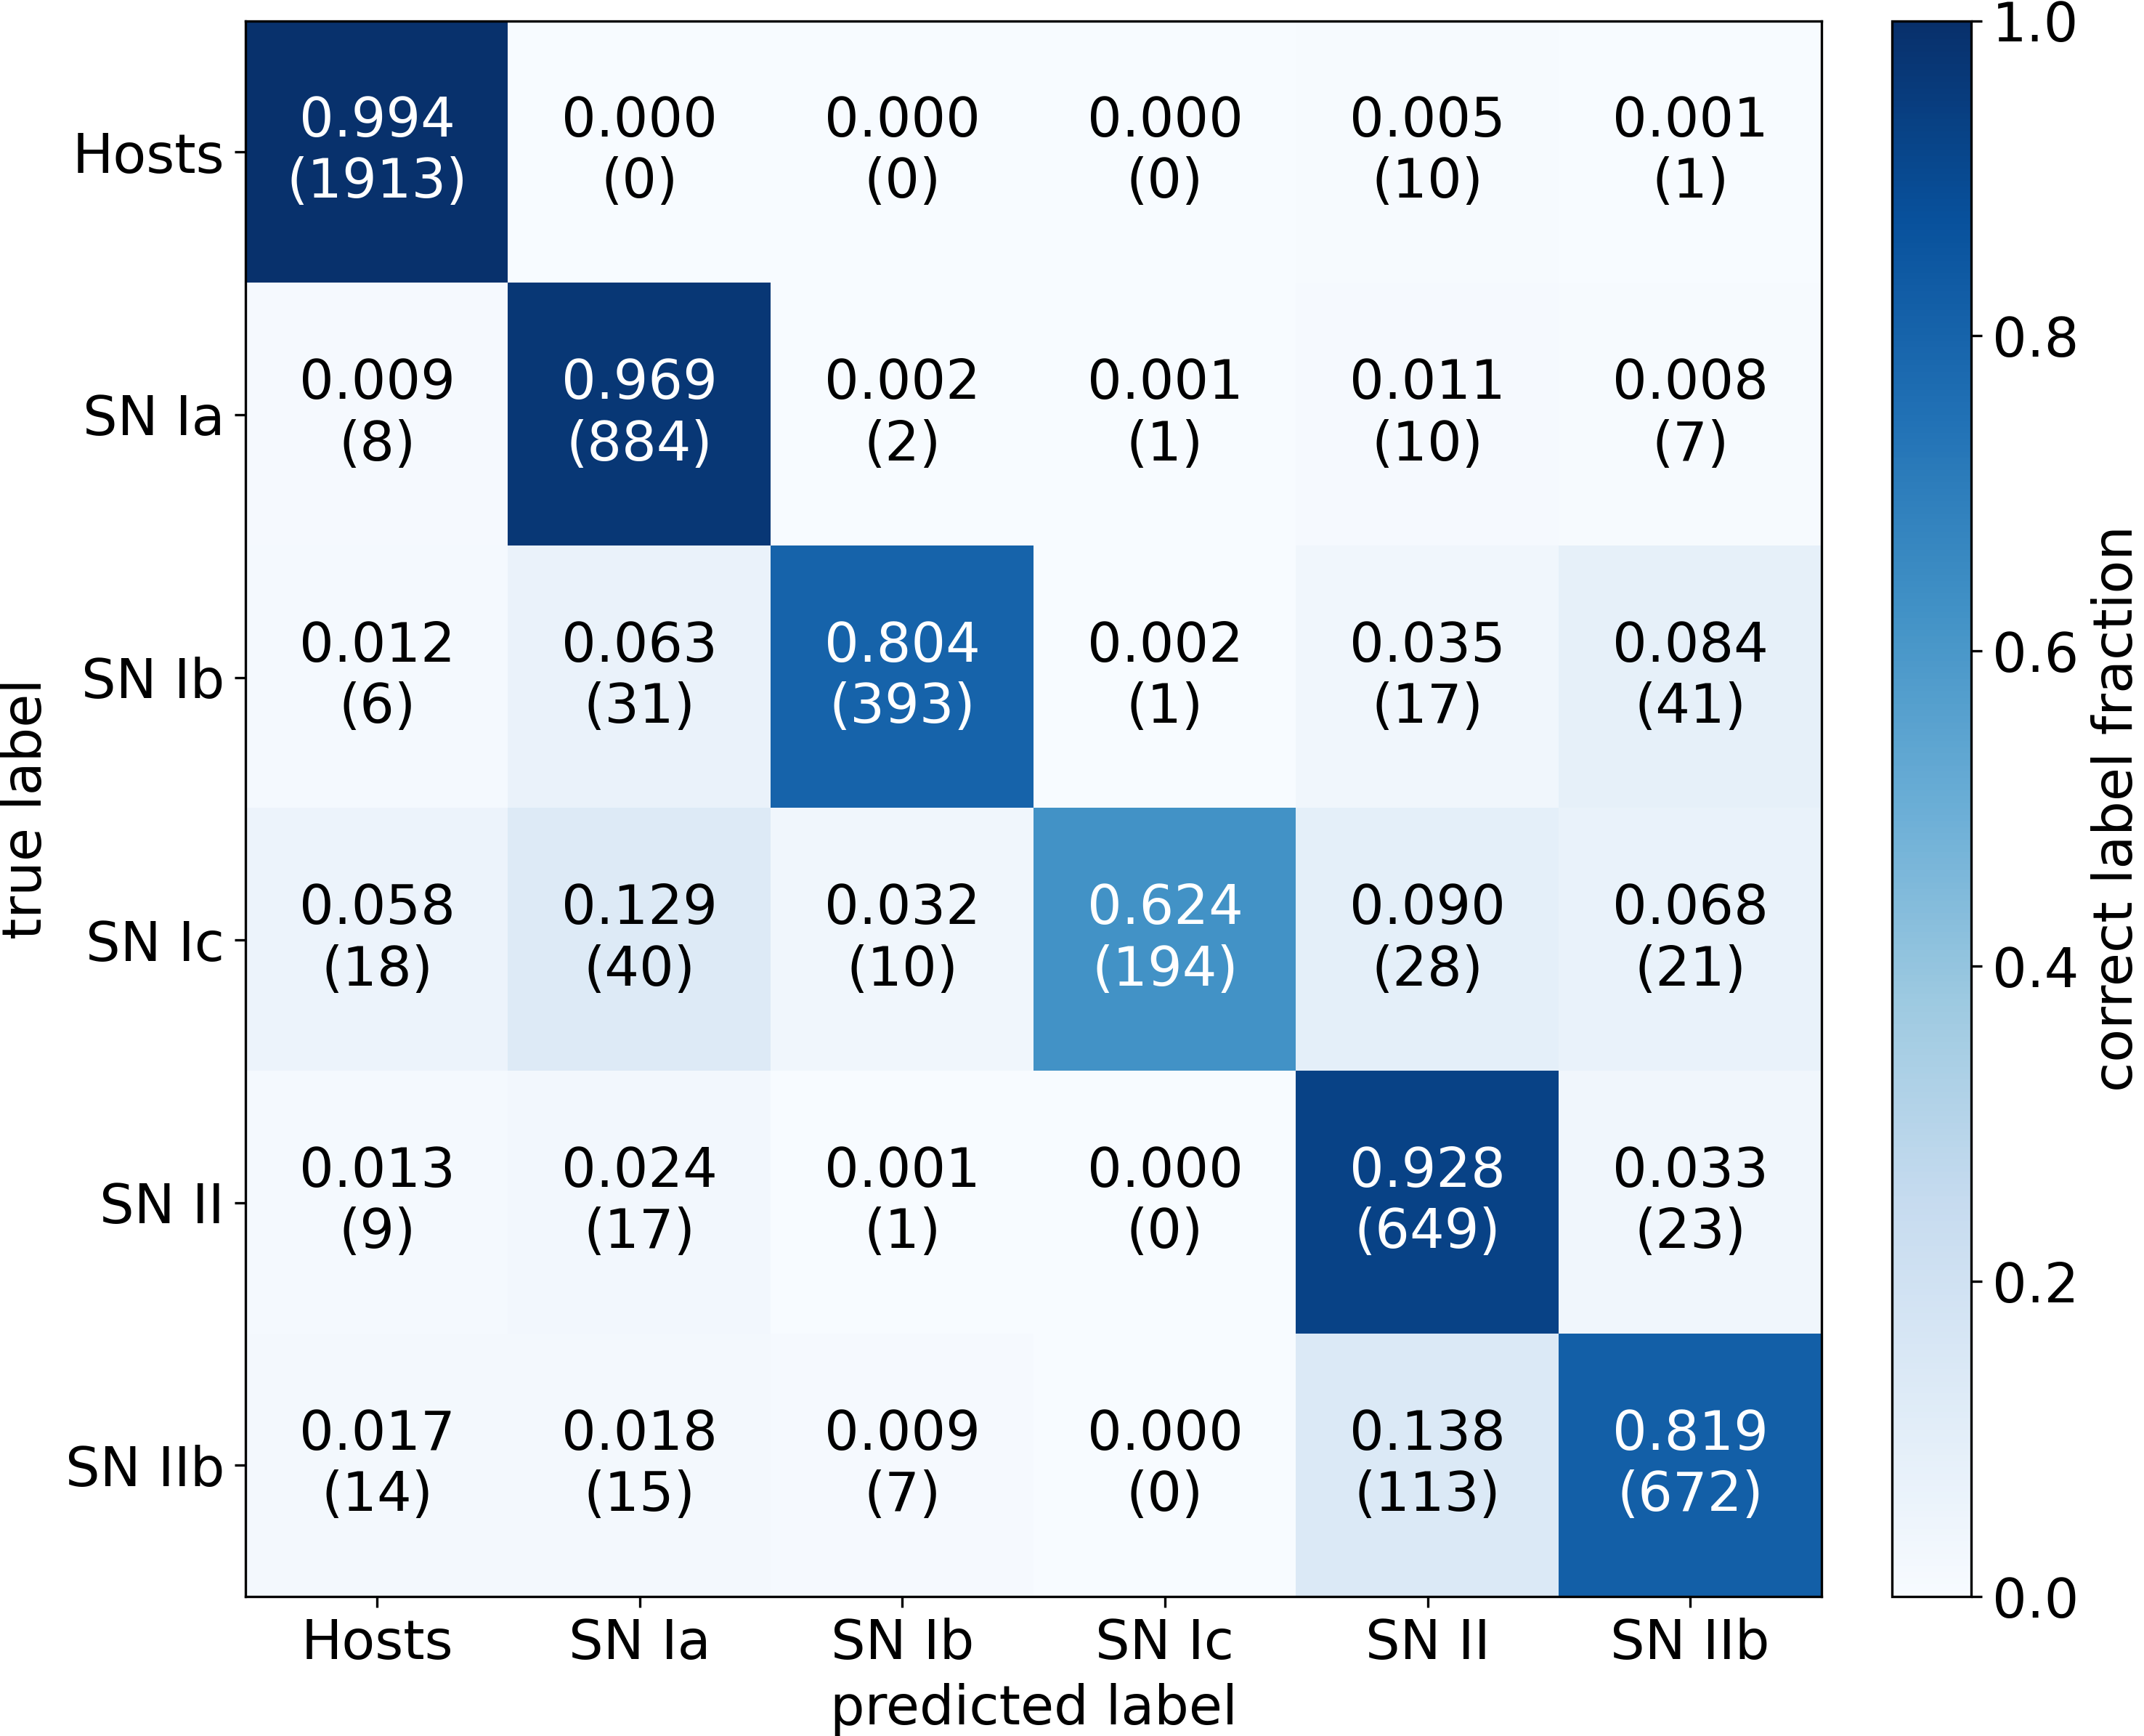
\includegraphics[height=4.3cm]{figures/v1_real/vit_model_V1_original_redocm999999_e31.png}
    \caption[Spectral ViT V1 Diagnostics: 99.9999\% Cut]{Spectral ViT V1 Diagnostics: ROC Curve (left) and Confusion Matrix (right) with a 99.9999\% confidence
    cut \label{fig:v1_999999_qual}}
\end{figure}

% \clearpage
\section{Spectral ViT V2: Specialized Classifier}
\begin{figure}[b!]
    \centering
    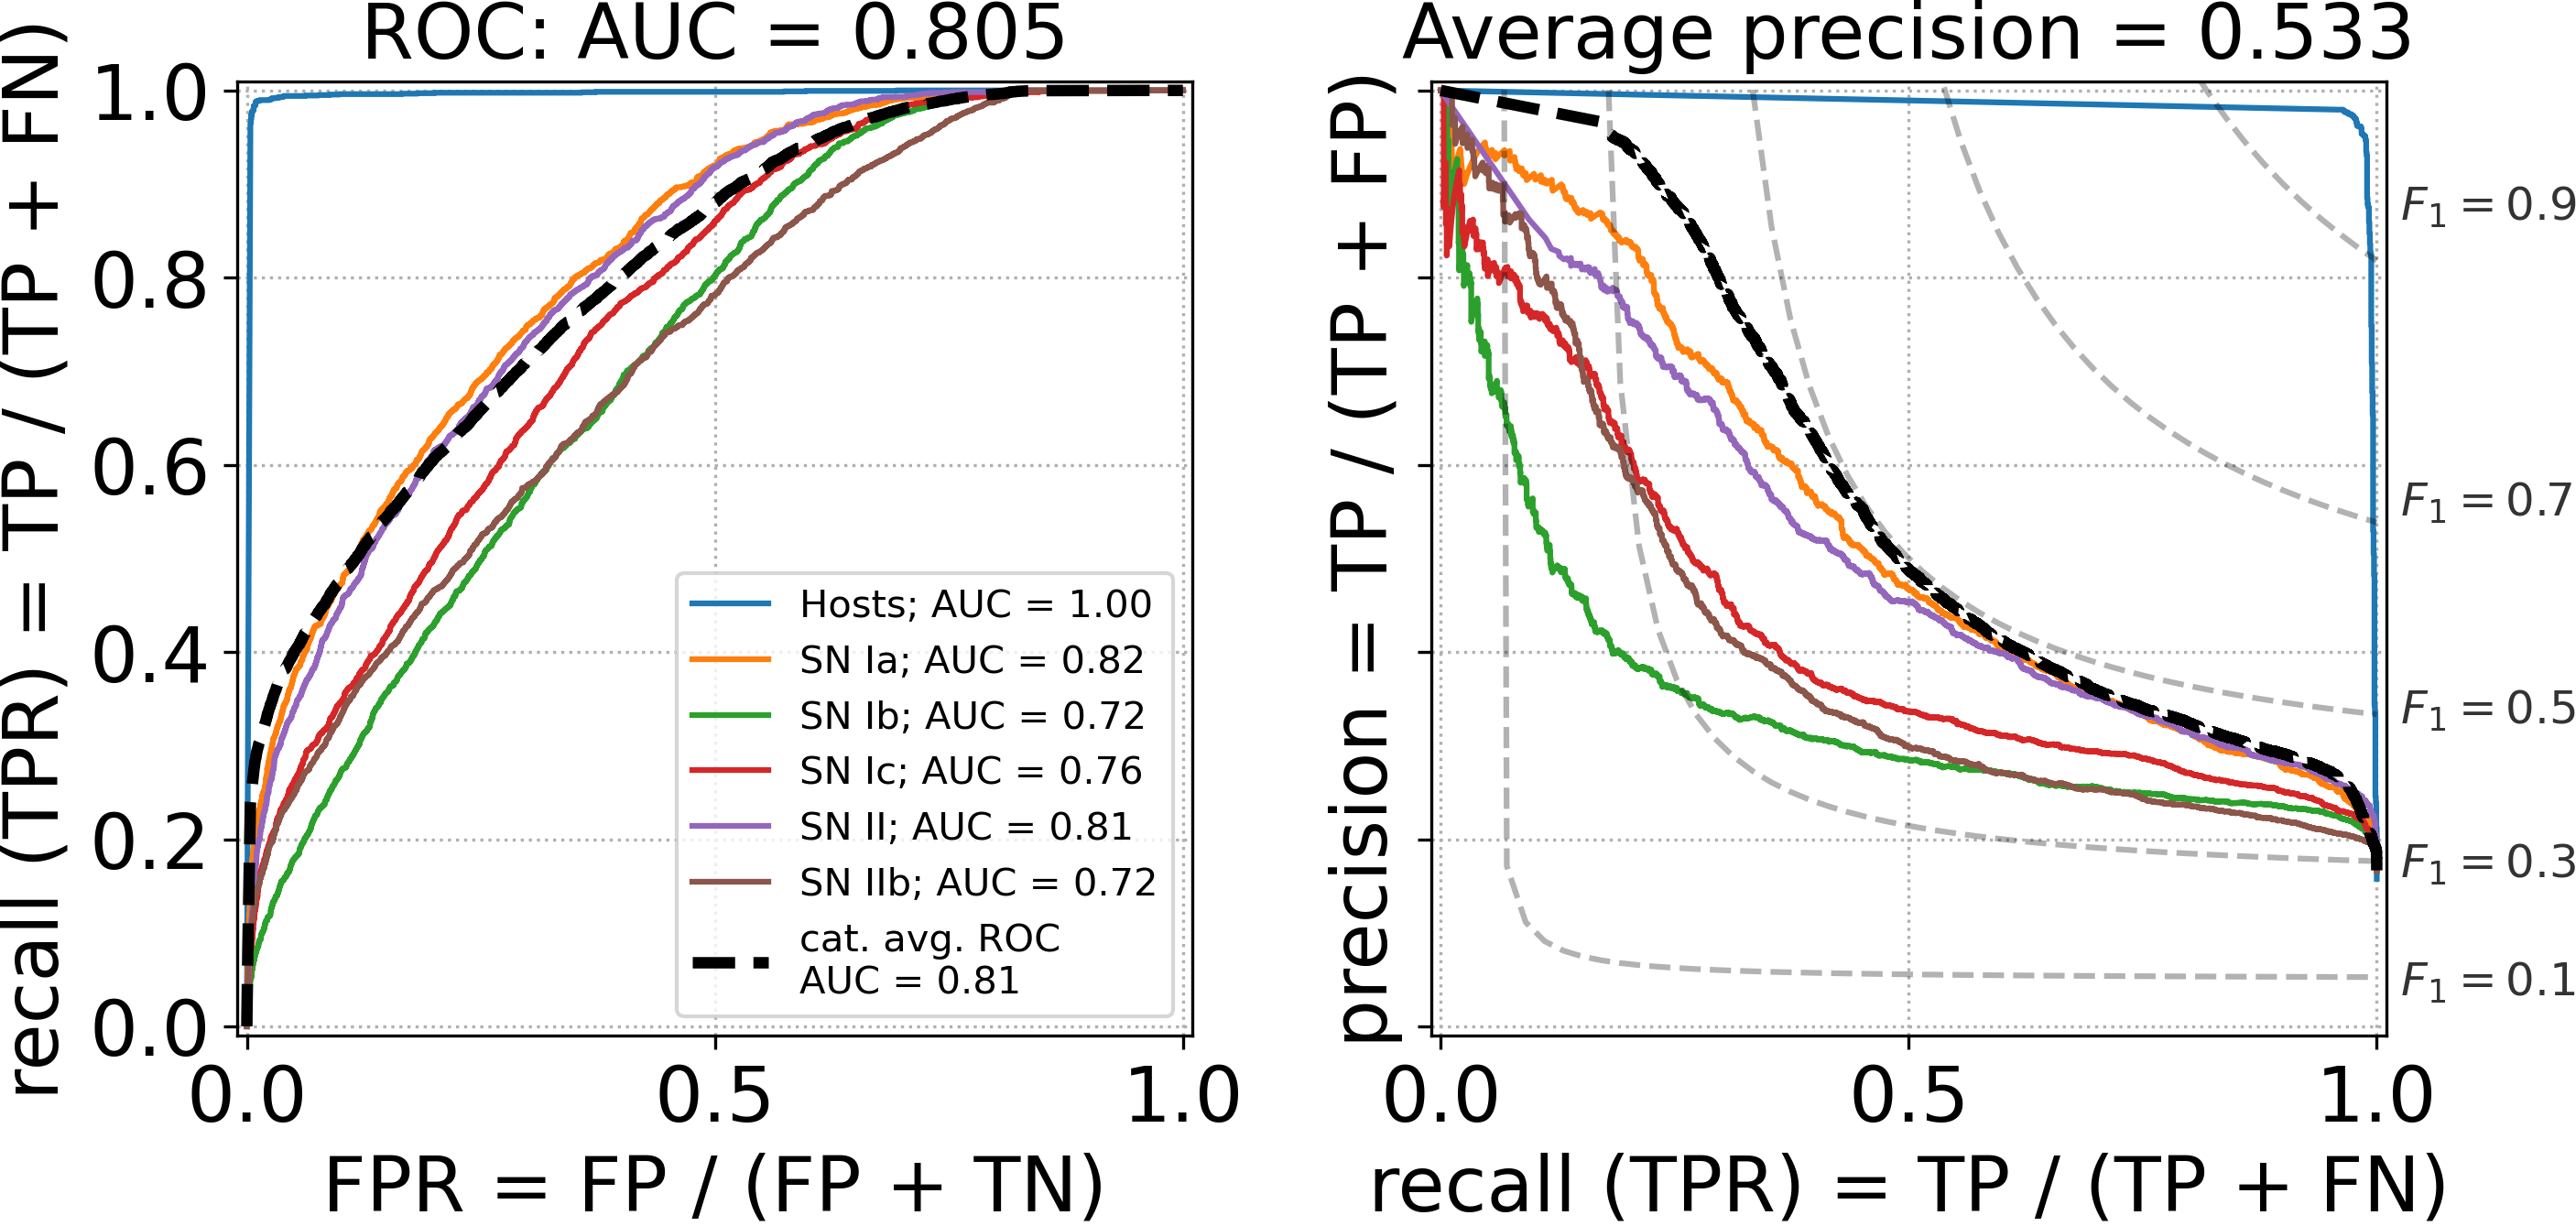
\includegraphics[height=4.3cm]{figures/v2_real/vit_model_V2rocfulle_e26.png}
    \quad
    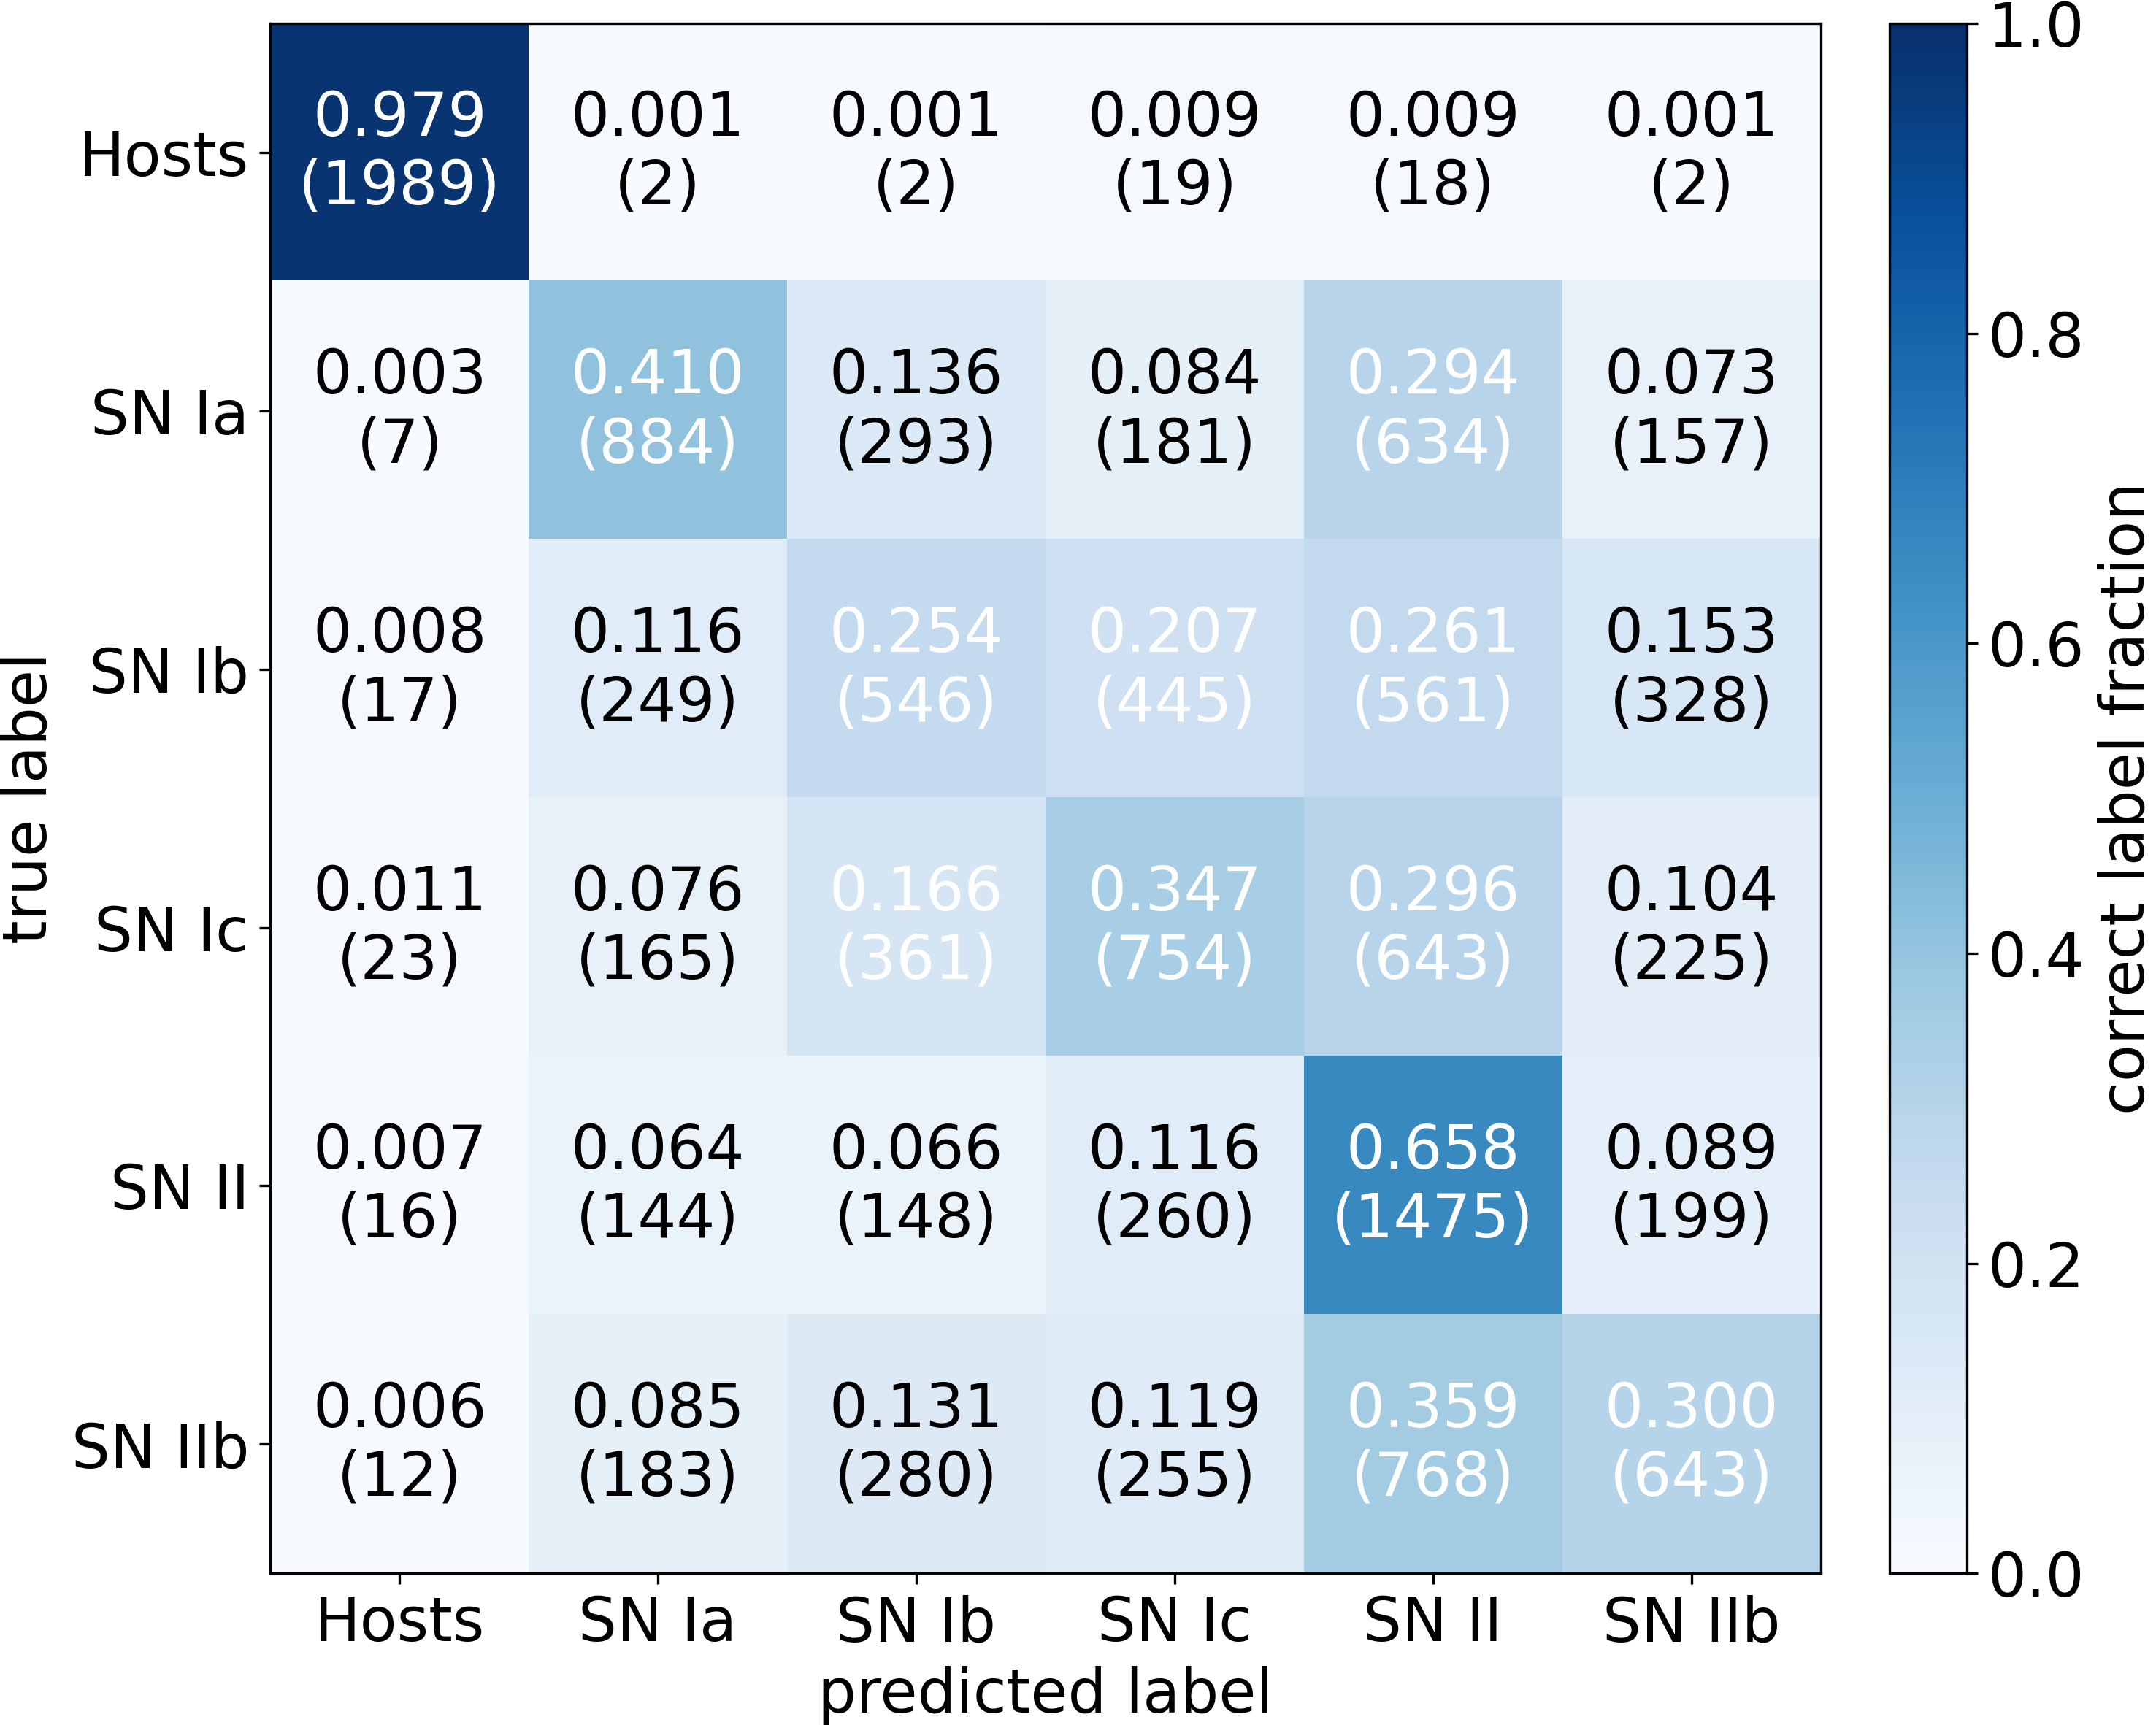
\includegraphics[height=4.3cm]{figures/v2_real/vit_model_V2cmfull_e26.png}
    \caption[Spectral ViT V2 Diagnostics]{Spectral ViT V2 Diagnostics: ROC Curve (left) and Confusion Matrix (right)\label{fig:v2_qual}}
\end{figure}
The goal of the Spectral ViT V2 was to see if the dependence on the redshift fit 
provided by the DESI pipeline could be removed. The validation set was the same size 
as the V1 validation set, 12888 specra. The ROC curve and confusion matrix are shown
in Figure~\ref{fig:v2_qual}. Classification of SNe and non-SNe is still very good,
with an AUC of 1.0, but the other classes are not classified as well, resulting in 
an overall AUC of 0.805 and a lower average precision of 53.3\%. 


Similar to the CNN, on a 99\% confidence cut, only 34\% of the original predictions
remain (Figure~\ref{fig:v2_max}). The AUC score and average precision both increase, as shown in Figure~\ref{fig:v2_99_qual}, 
but the important metric is the number of positive predictions made. The ViT, 
despite not looking at spectra in the rest frame, was still able to identify more 
Host and SN II spectra than the CNN, but not as many of the other spectra. 


\begin{figure}[t!]
    \centering
    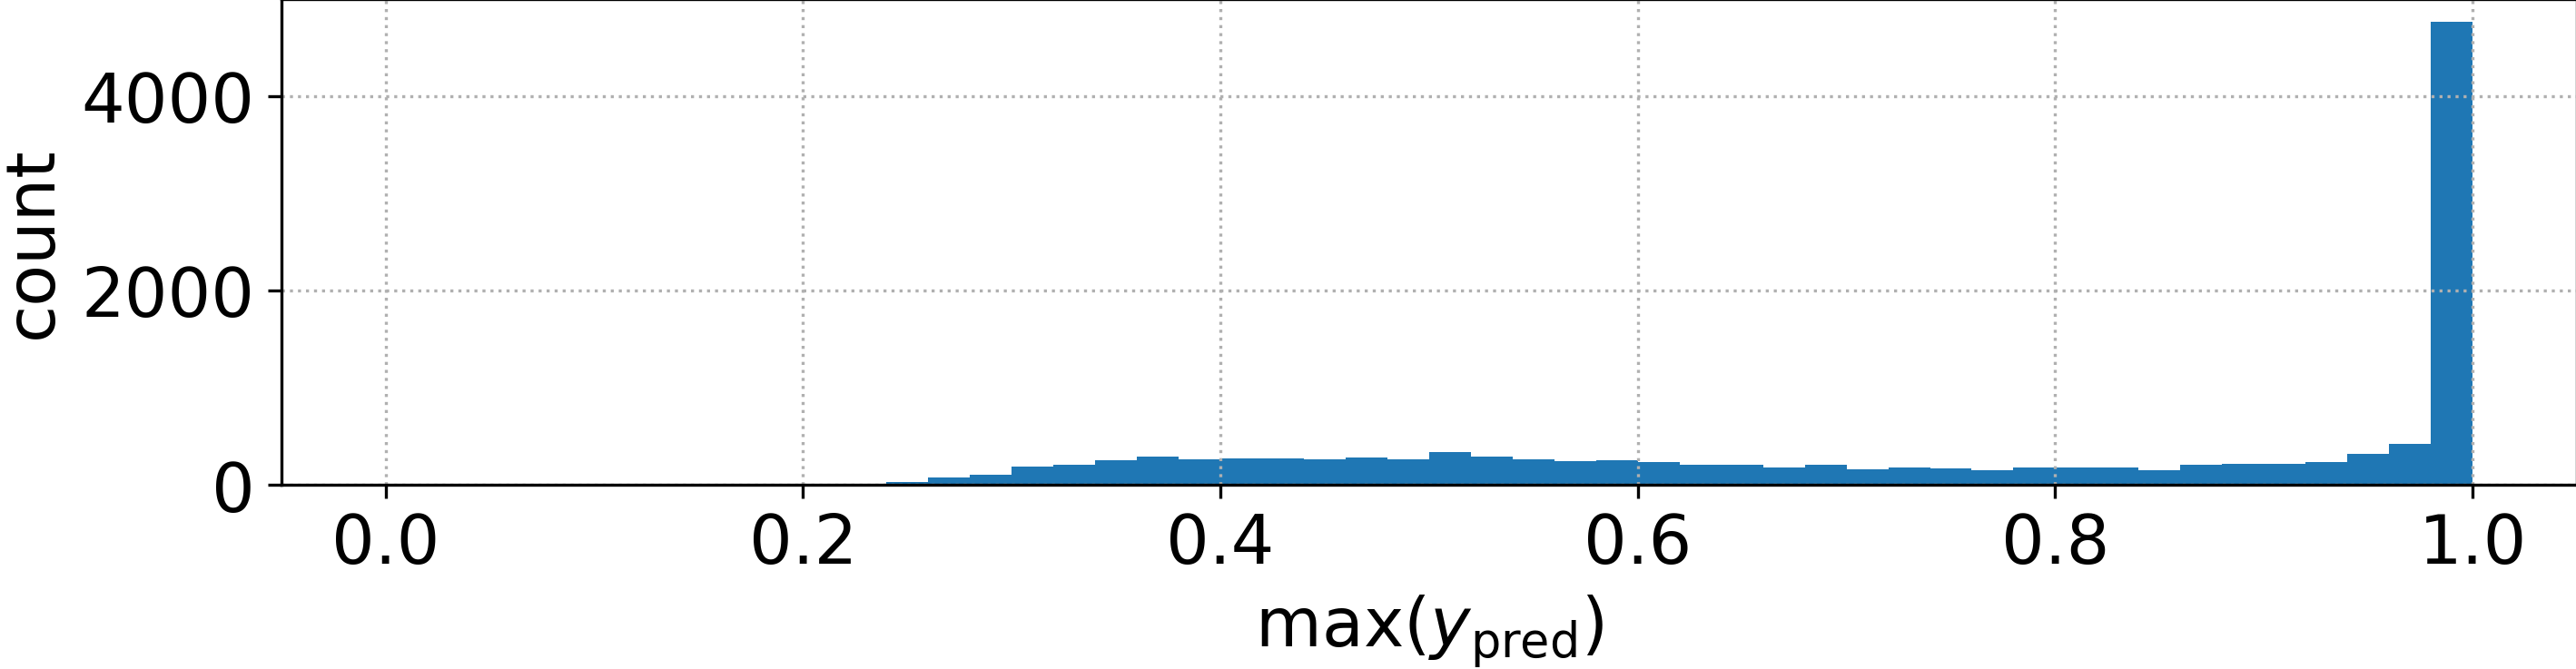
\includegraphics[width=0.8\textwidth]{figures/v2_real/vit_model_V2max_ypred_26.png}
    \caption[Spectral ViT V2 Confidence]{Max value of the output vector from the Spectral ViT V2.\label{fig:v2_max}}
\end{figure}

\begin{figure}[b!]
    \centering
    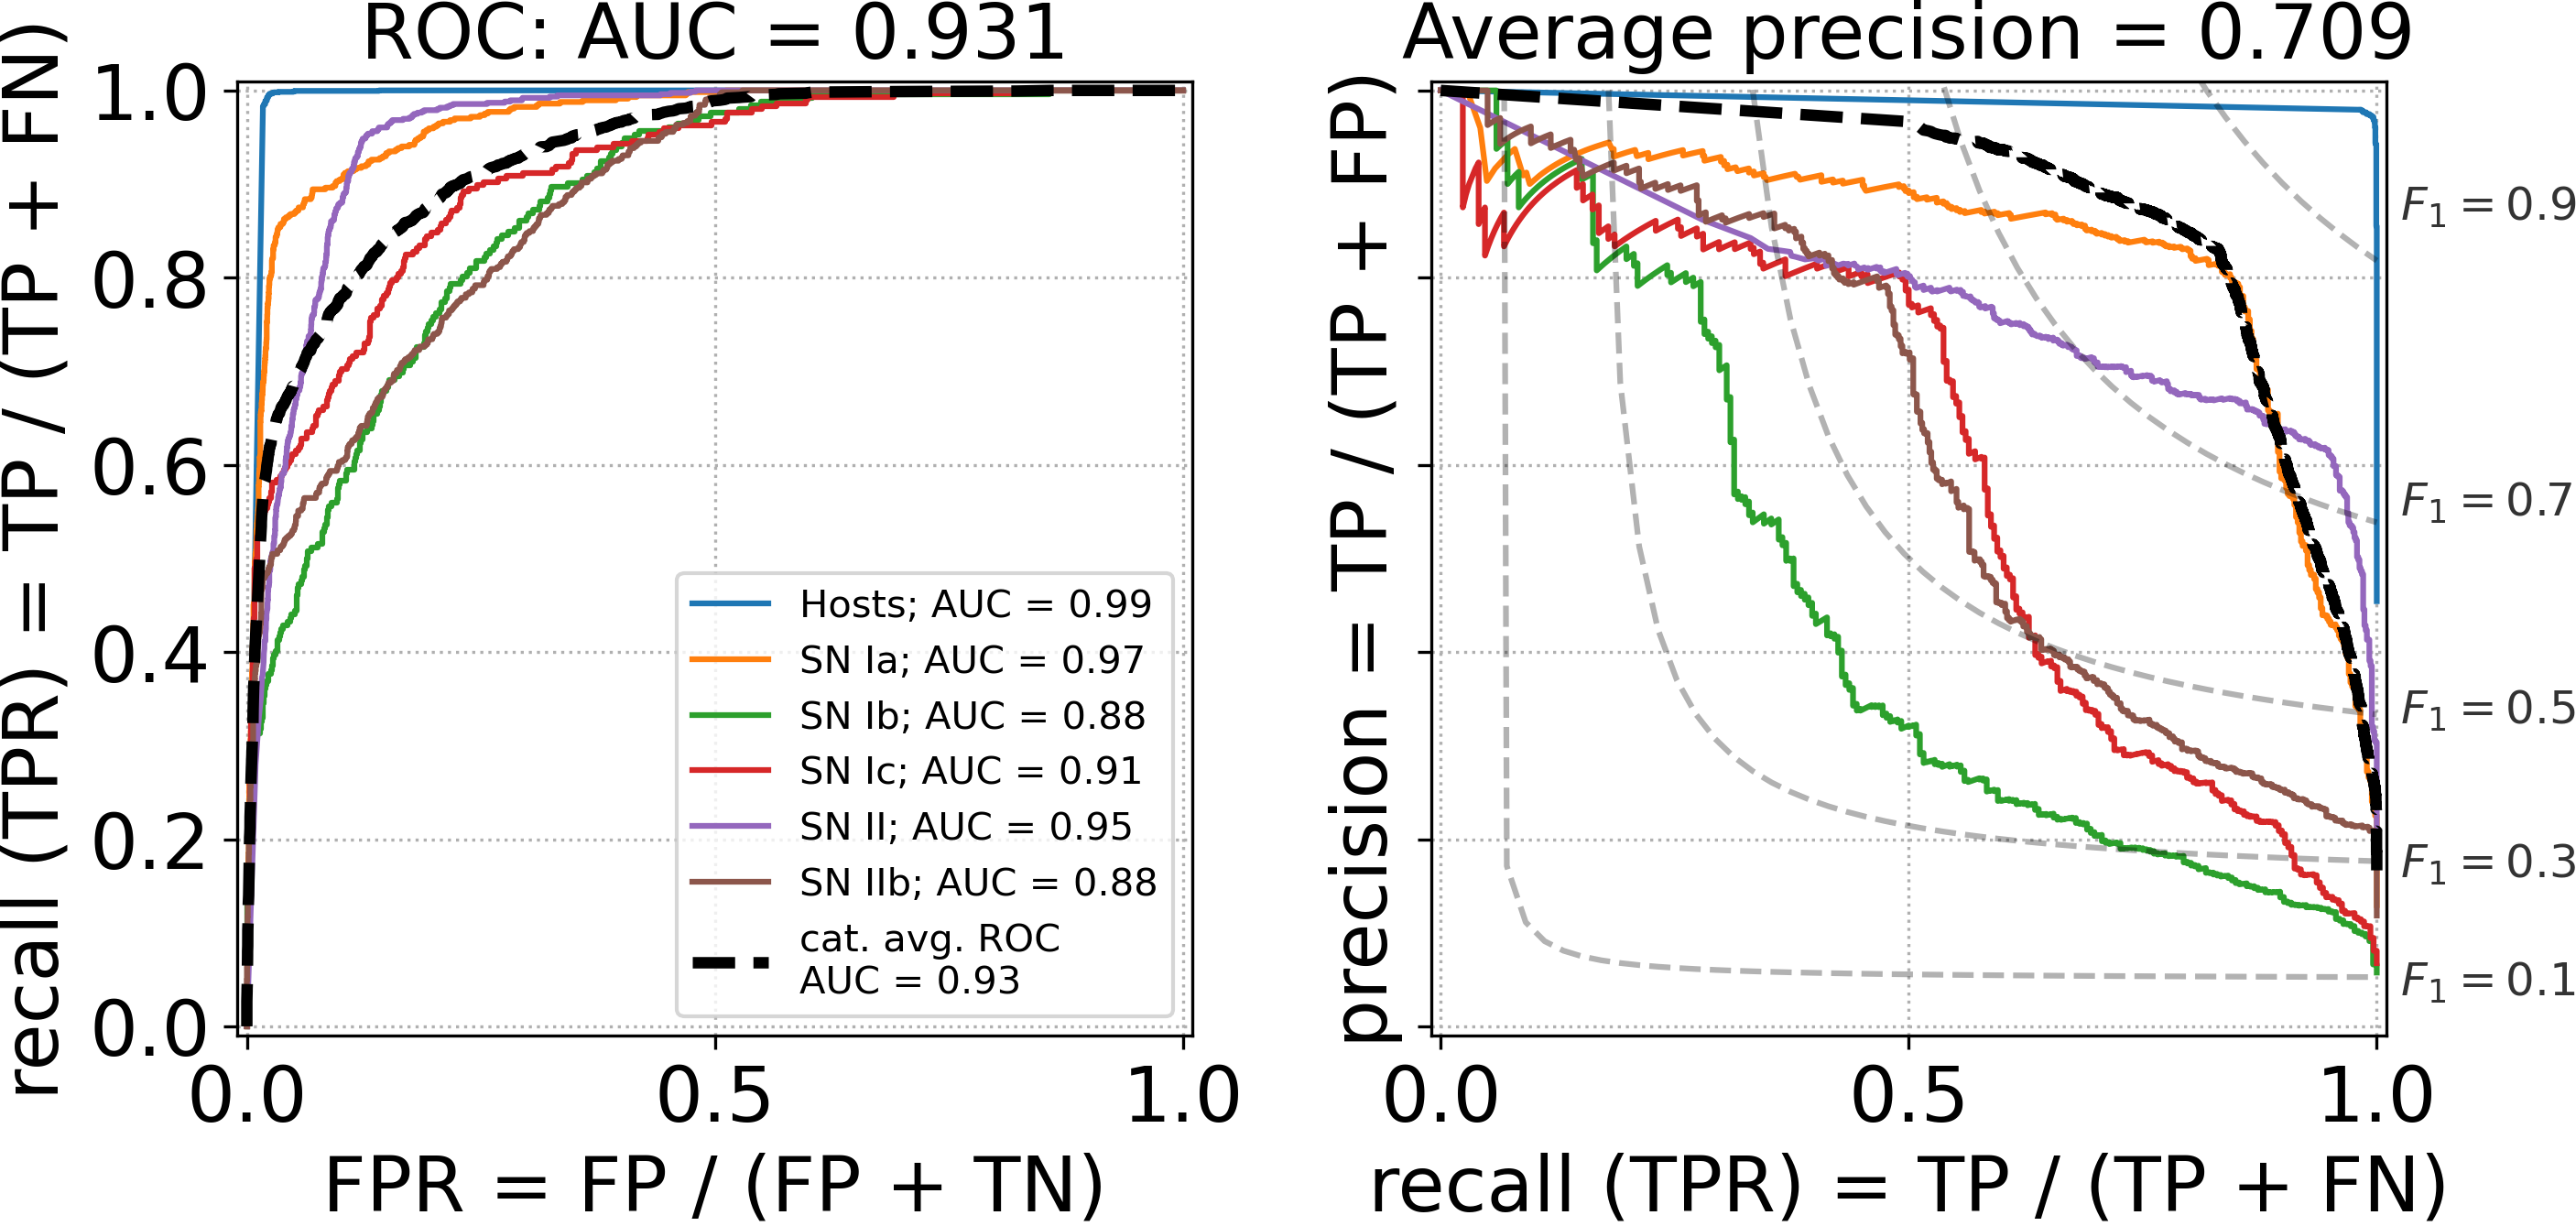
\includegraphics[height=4.3cm]{figures/v2_real/vit_model_V2roc99_e26.png}
    \quad
    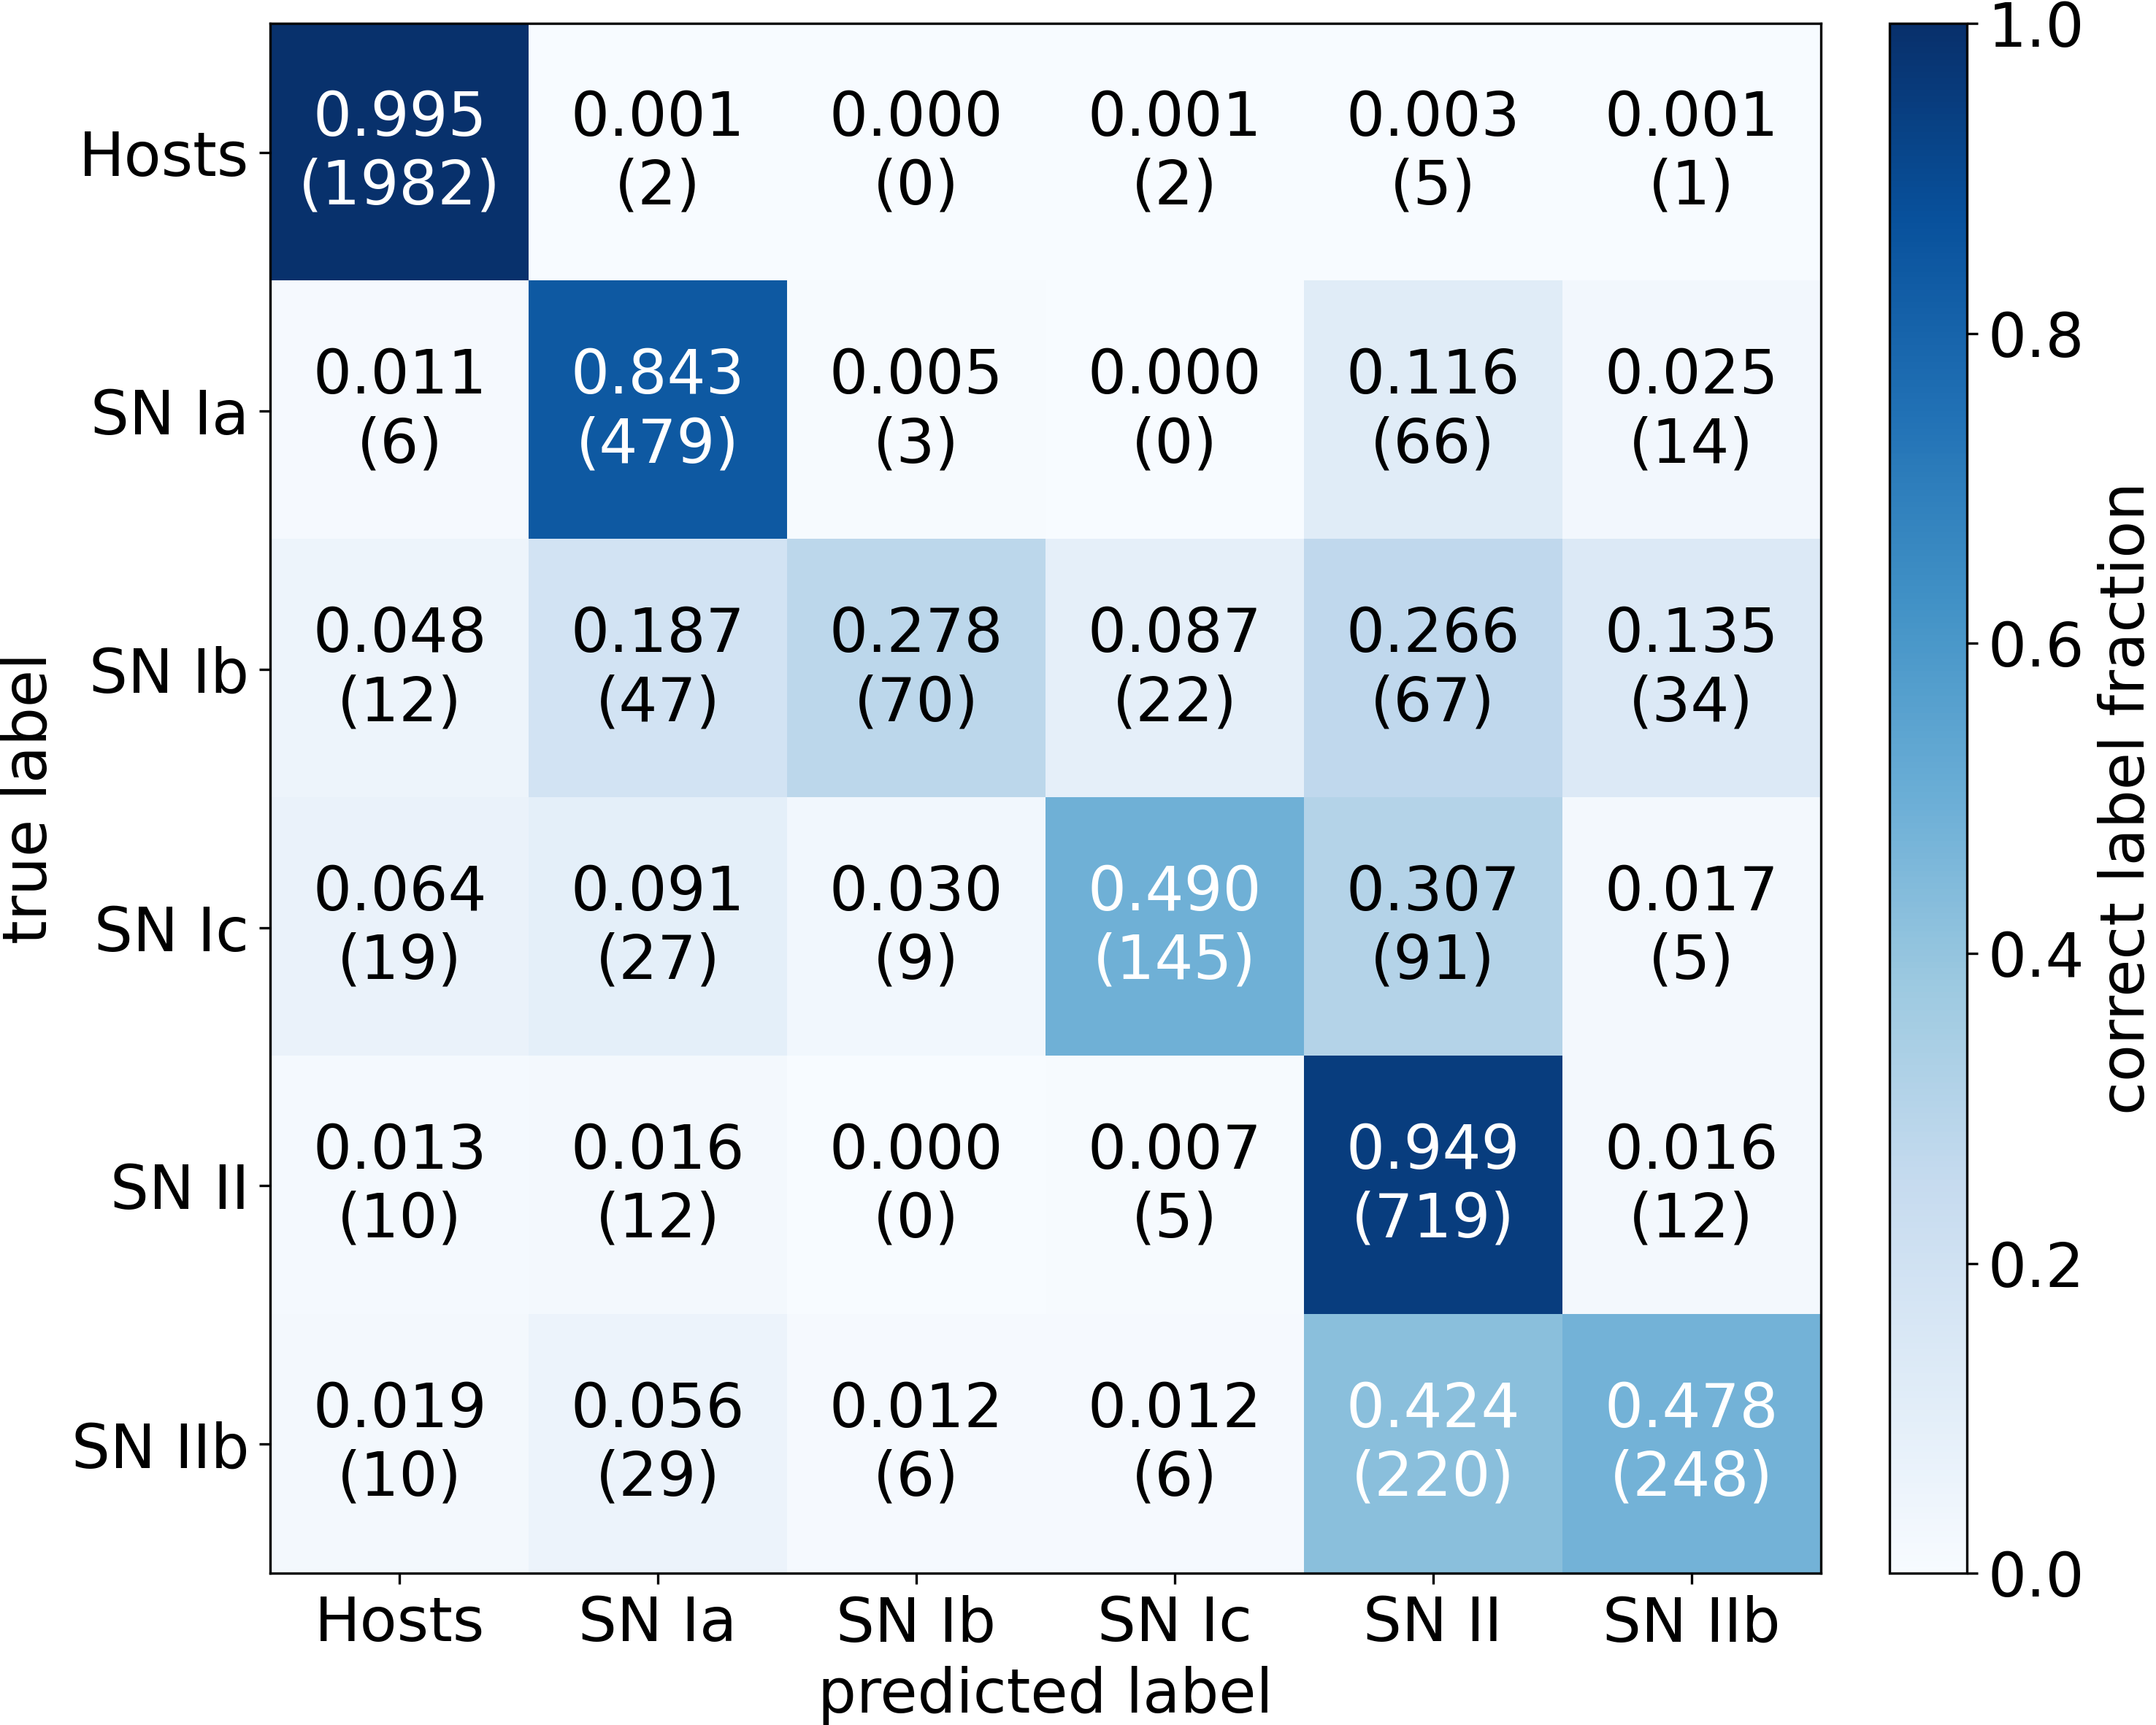
\includegraphics[height=4.3cm]{figures/v2_real/vit_model_V2cm99_e26.png}
    \caption[Spectral ViT V2 Diagnostics: 99\% Cut]{Spectral ViT V2 Diagnostics: ROC Curve (left) and Confusion Matrix (right) with a 99\% confidence
    cut\label{fig:v2_99_qual}}
\end{figure}

This, combined with the lower AUC score, indicates that the ViT V2 is not a suitable 
replacement for the ViT V1 for the purposes of SNe sub-type classification. However, the ViT V2
is still able to differentiate SNe and non-SNe spectra with high accuracy, so alternative uses 
can be derived from the existing classifier. 

\subsection{Alternative Applications of the V2 Classifier}

\subsubsection{Binary Classifier}

The most obvious use for a classifier capable of identifying the presence, or lack thereof, of a supernova 
with a high degree of accuracy is a binary classifier. To alter the predictions presented by the ViT 
for binary classification, the probabilities of all classes apart from 
non-SNe were summed. This resulted in a very high AUC score of 0.997, with a 
nearly perfect average precision of 98.7\% (Figure \ref{fig:v2_binary_qual}).
\begin{figure}[t!]
    \centering
    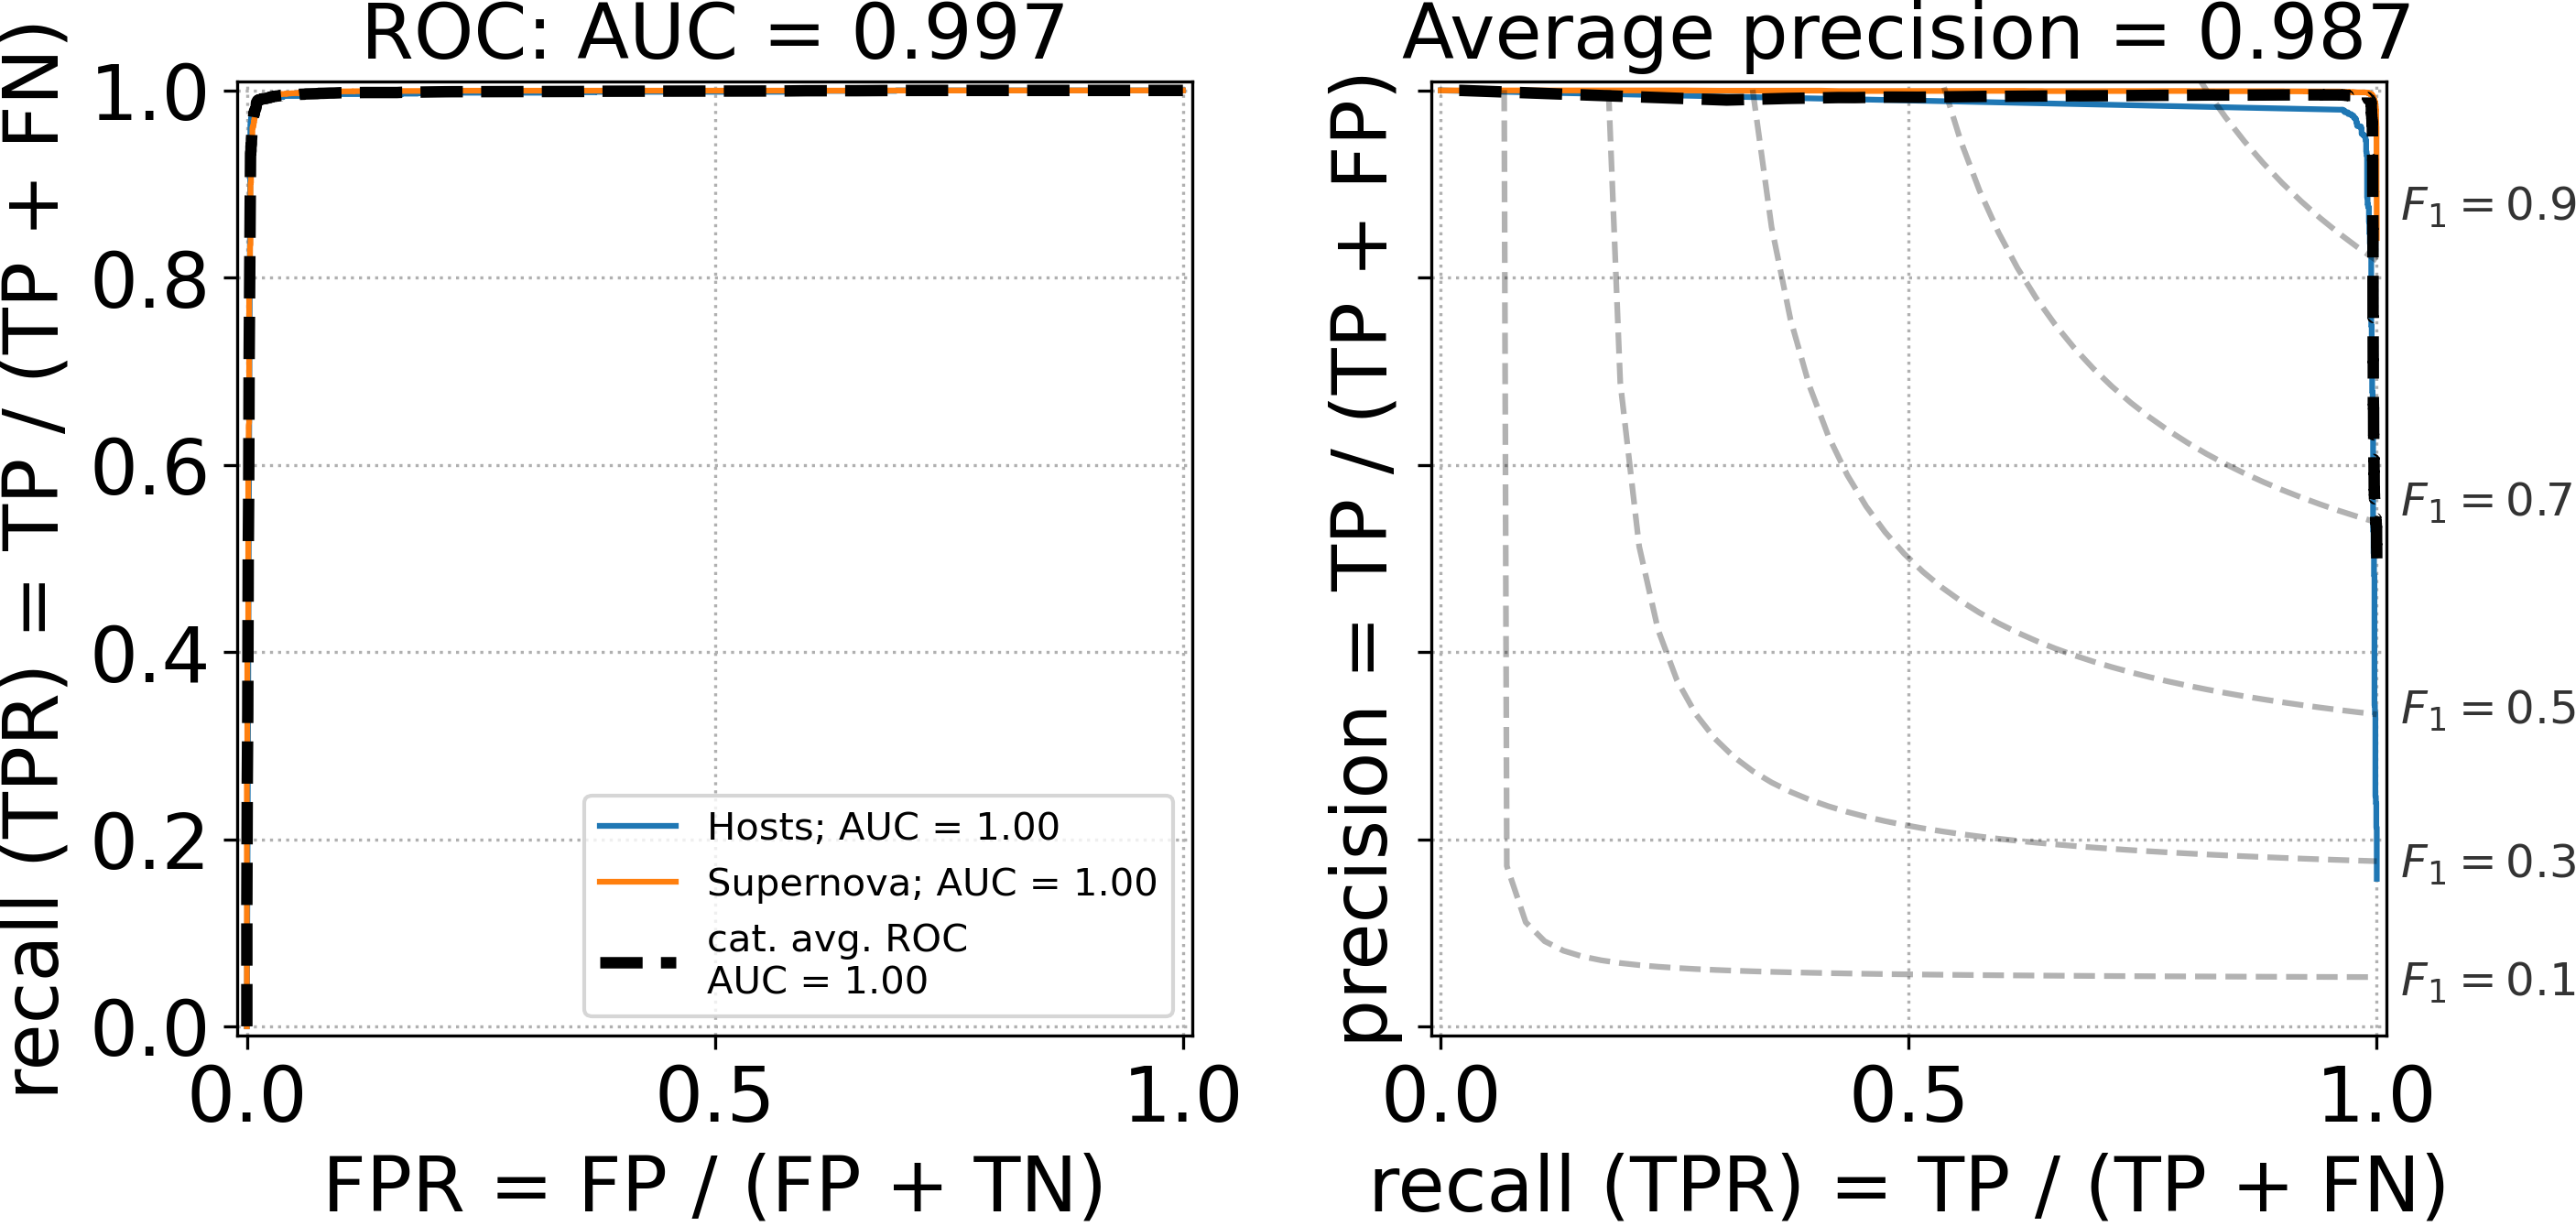
\includegraphics[height=4.2cm]{figures/v2_real/vit_model_V2rocfull_binary_e26.png}
    \quad
    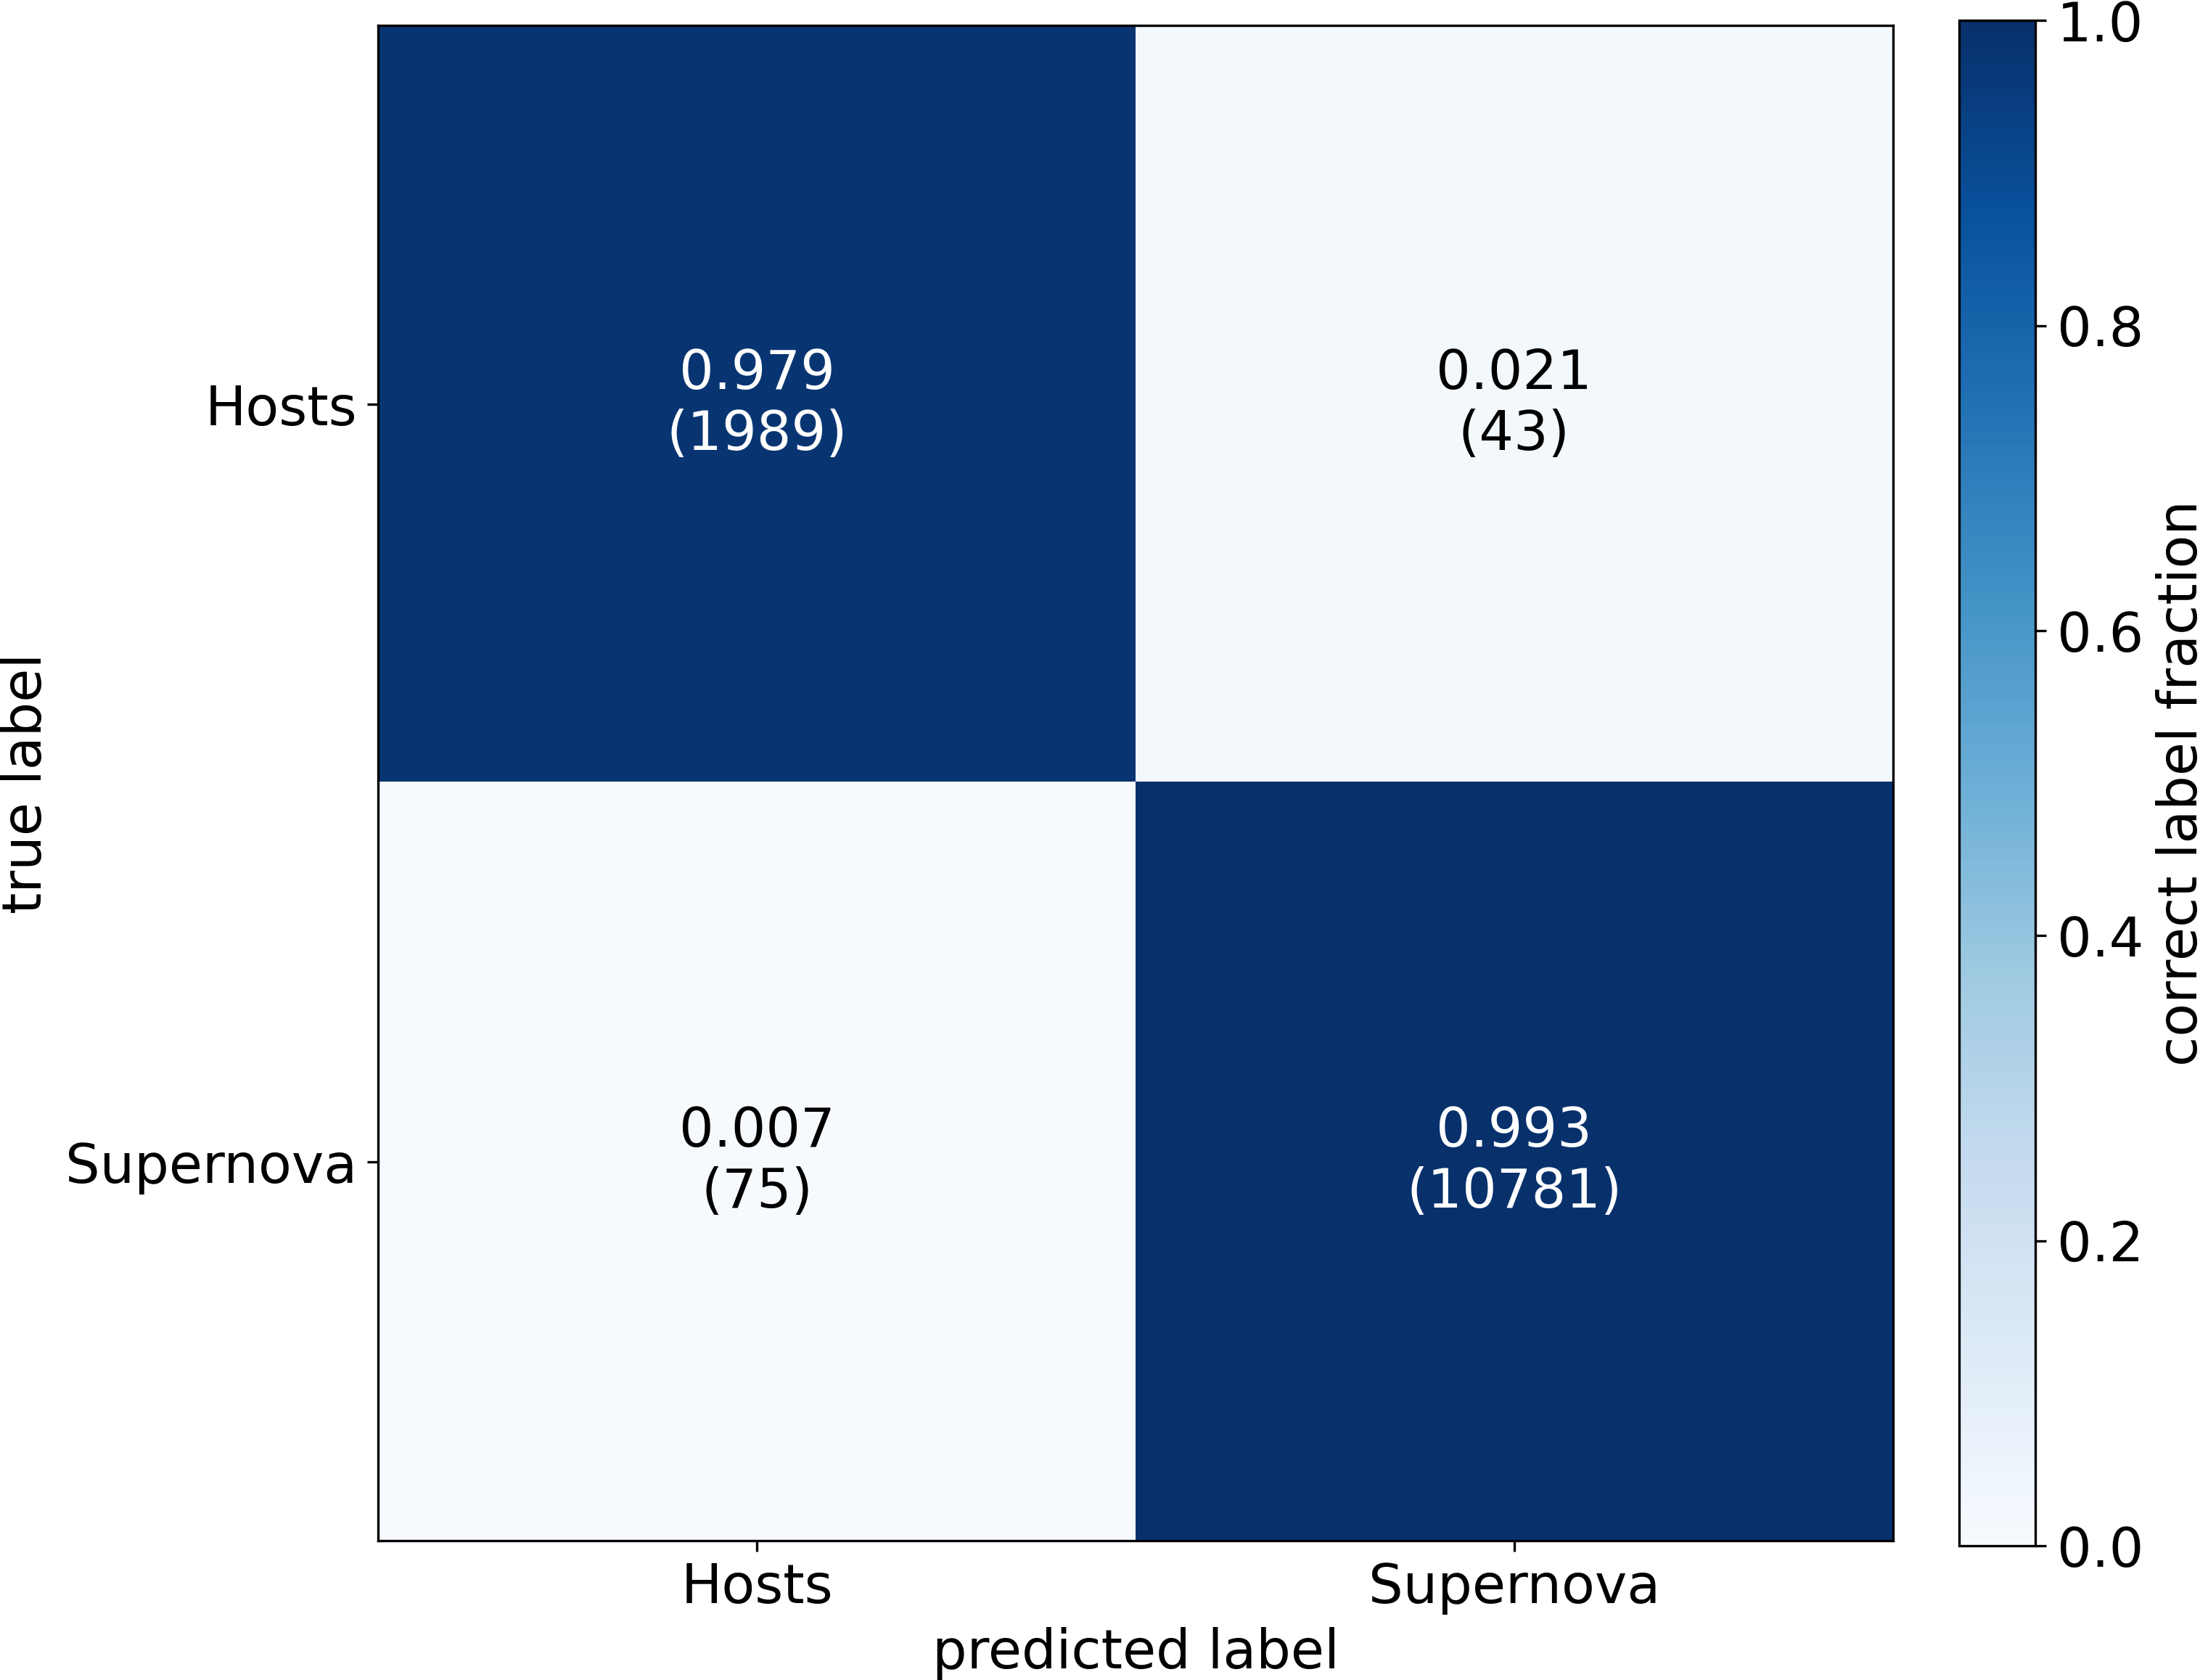
\includegraphics[height=4.2cm]{figures/v2_real/vit_model_V2cmfull_binary_e26.png}
    \caption[Spectral ViT V2 Binary Diagnostics]{Spectral ViT V2 Binary Diagnostics:
    ROC Curve (left) and Confusion Matrix (right)\label{fig:v2_binary_qual}}
\end{figure}
This, combined with the over 55\% of sample classifications having a prediction confidence of over 99.9999\%,
indicates the ViT V2's outstanding ability to act as a binary classifier for the presence of SNe.
% \begin{figure}[hb!]
%     \centering
%     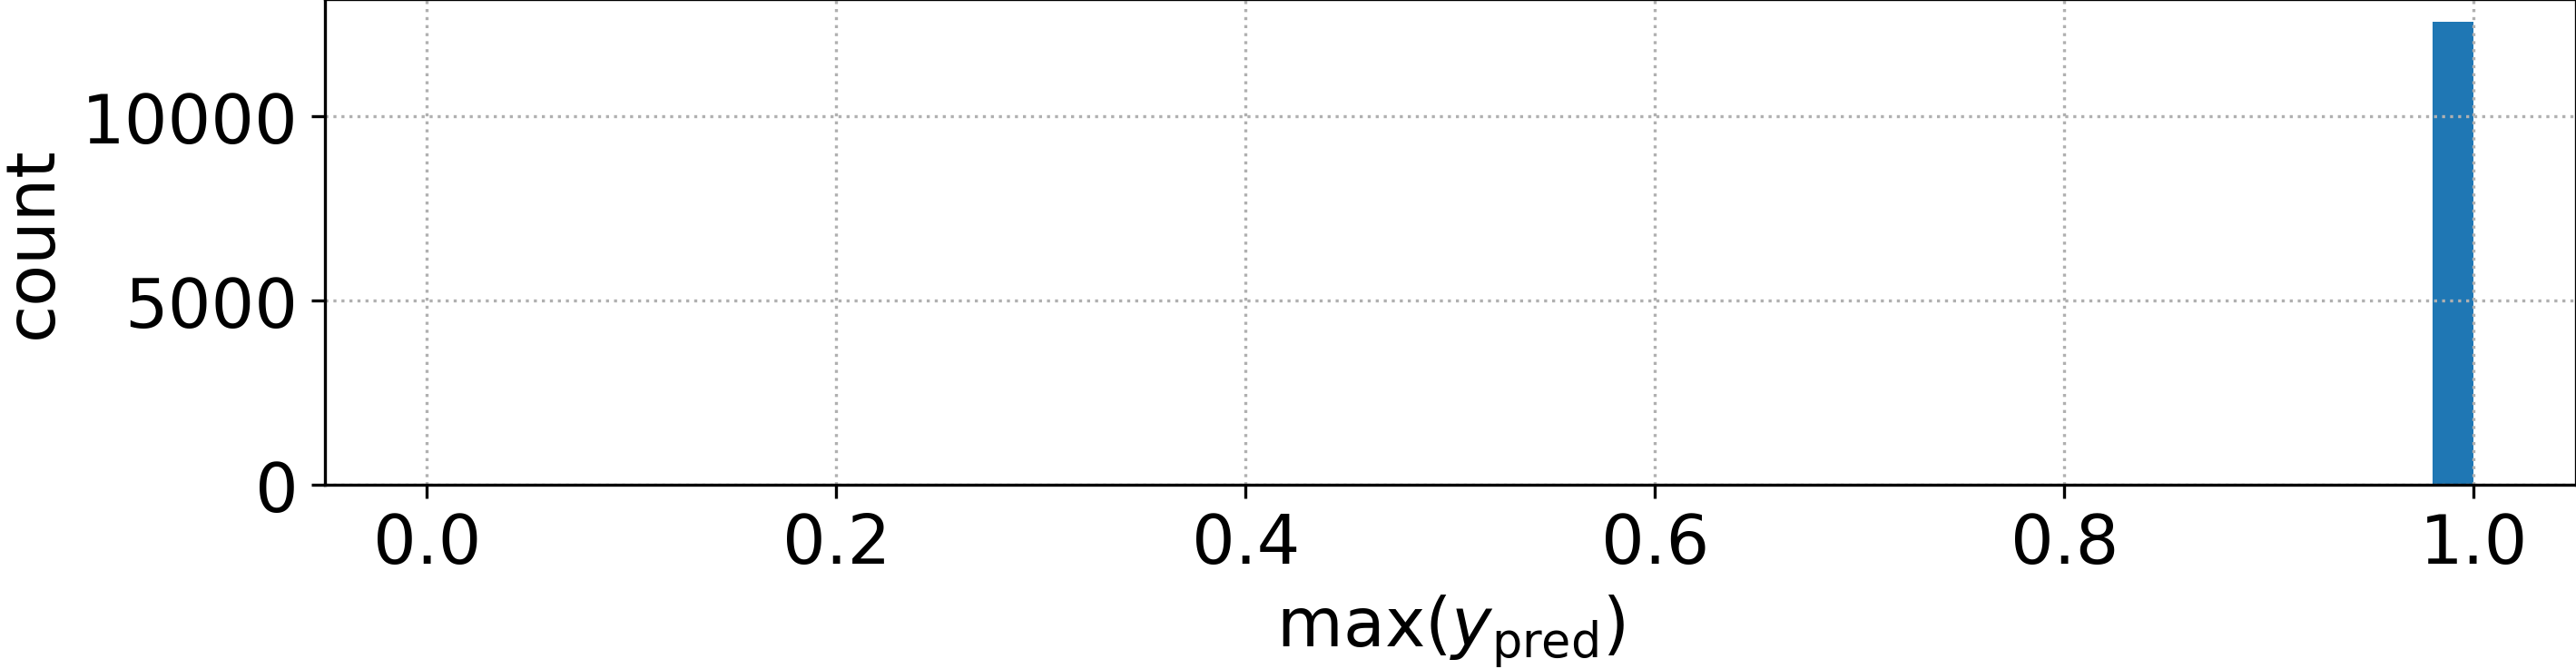
\includegraphics[width=0.8\textwidth]{figures/v2_real/vit_model_V2max_ypred_binary_26.png}
%     \caption[Spectral ViT V2 Confidence]{Max value of the output vector from the 
%     Spectral ViT V2 Binary Classification.\label{fig:v2_binary_max}}
% \end{figure}

\subsubsection{Progenitor and Type Classification}
\begin{figure}[htb!]
    \centering
    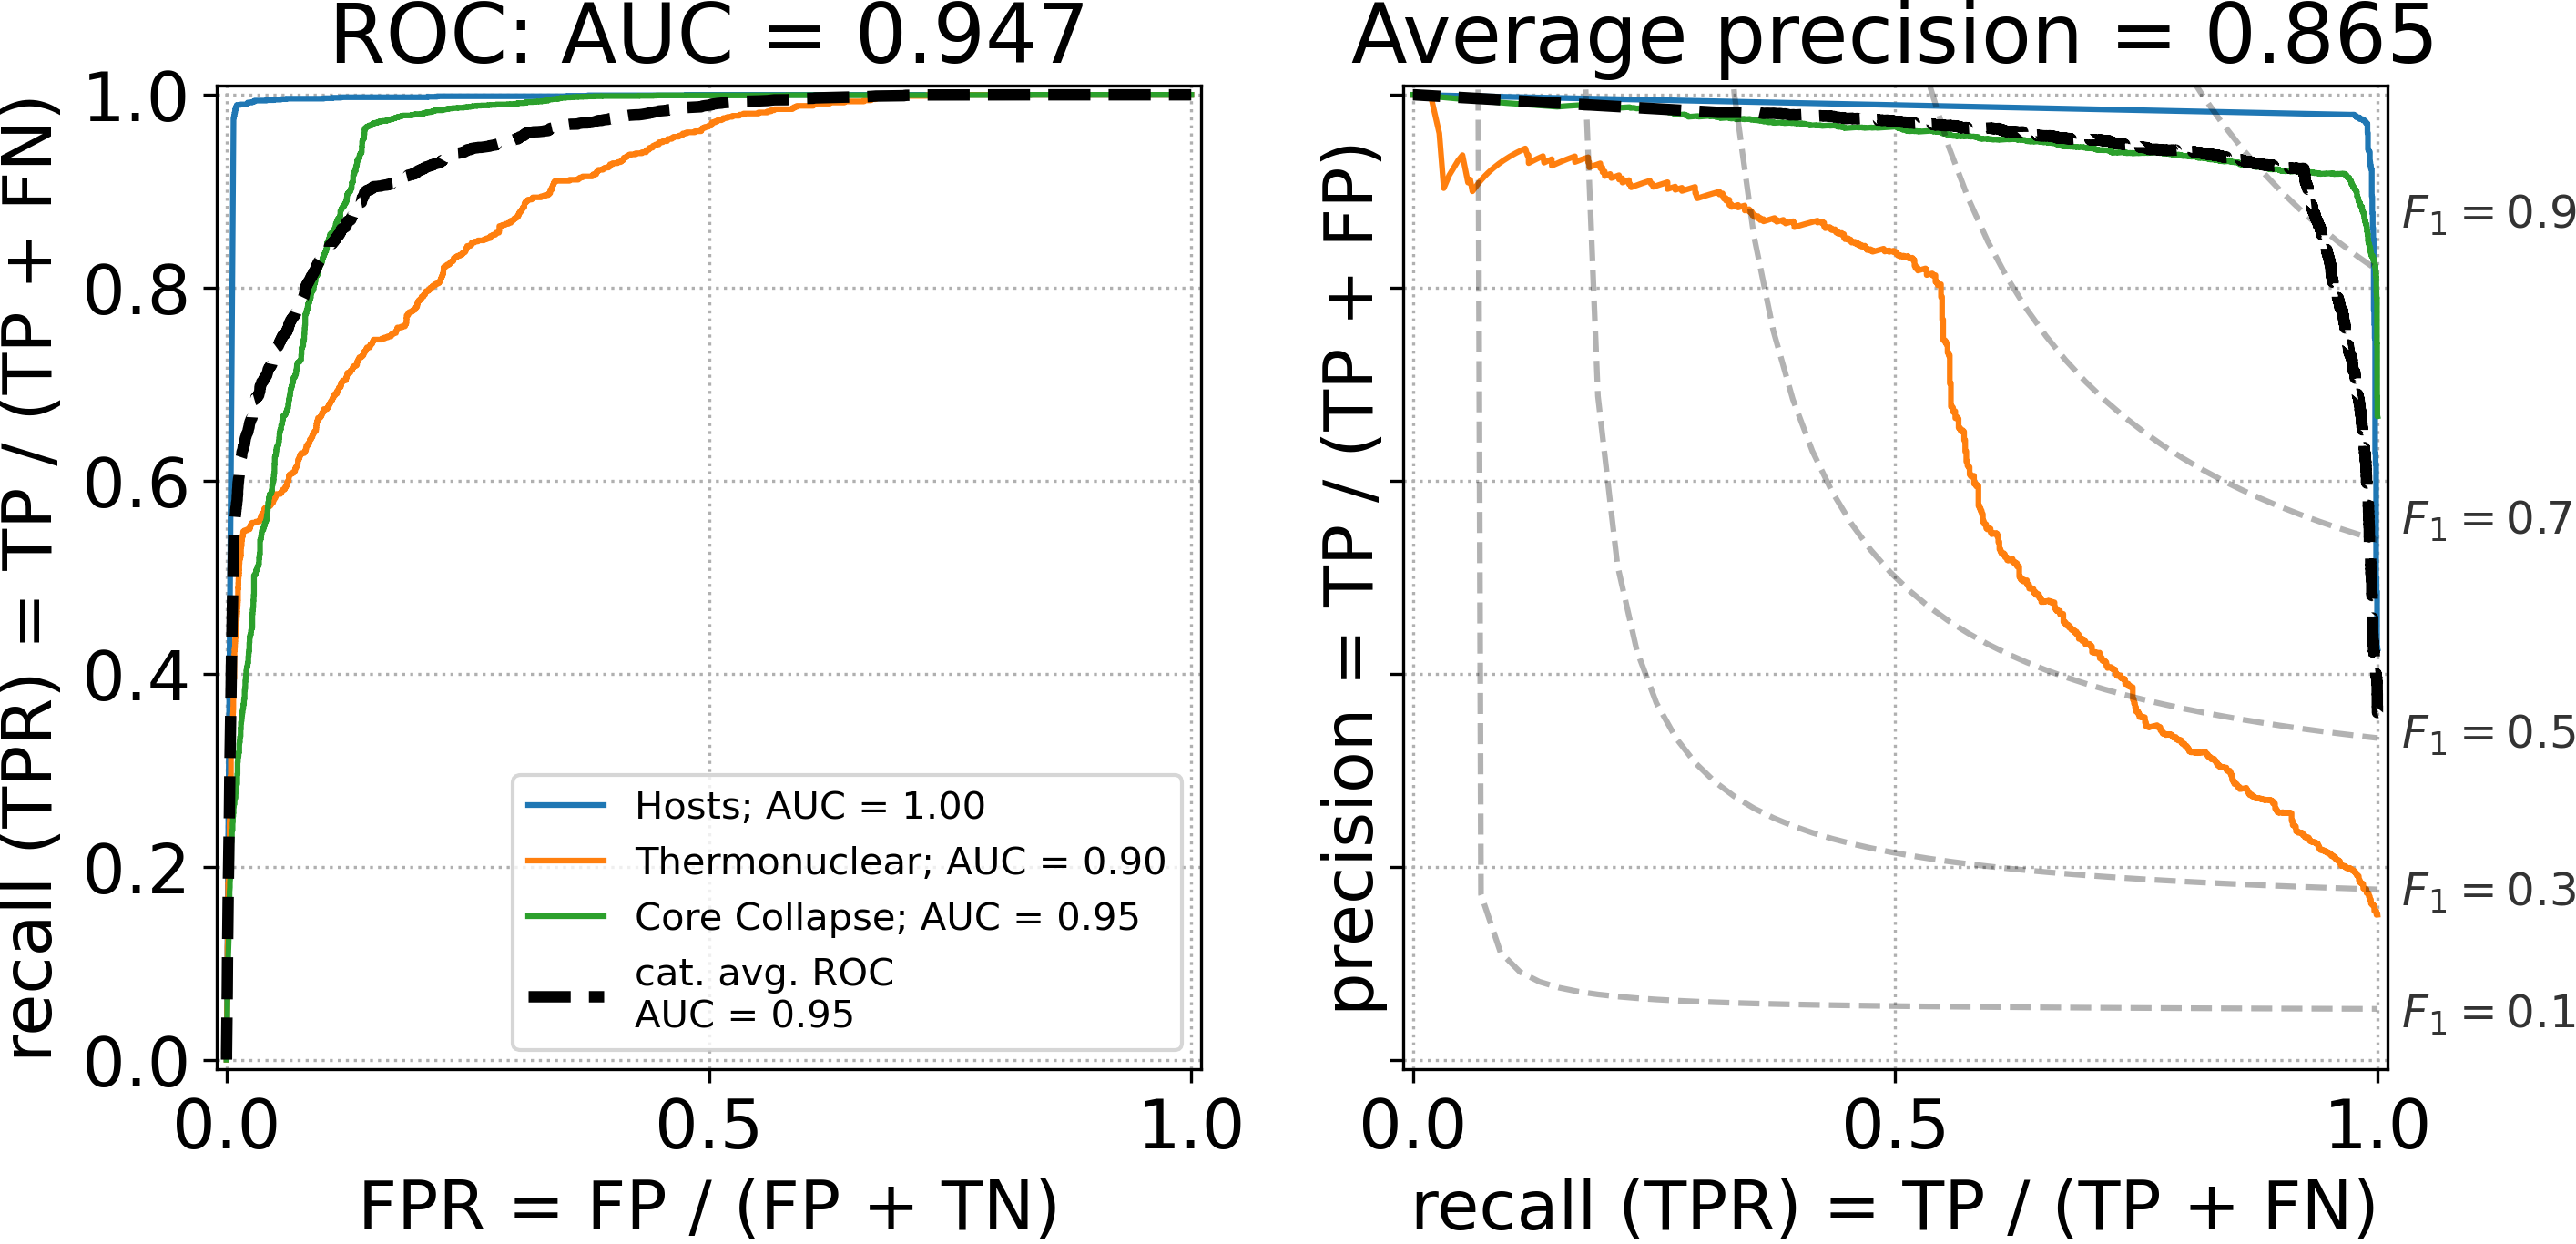
\includegraphics[height=4.1cm]{figures/v2_applications/vit_model_V2roc99_proj_e26.png}
    \quad
    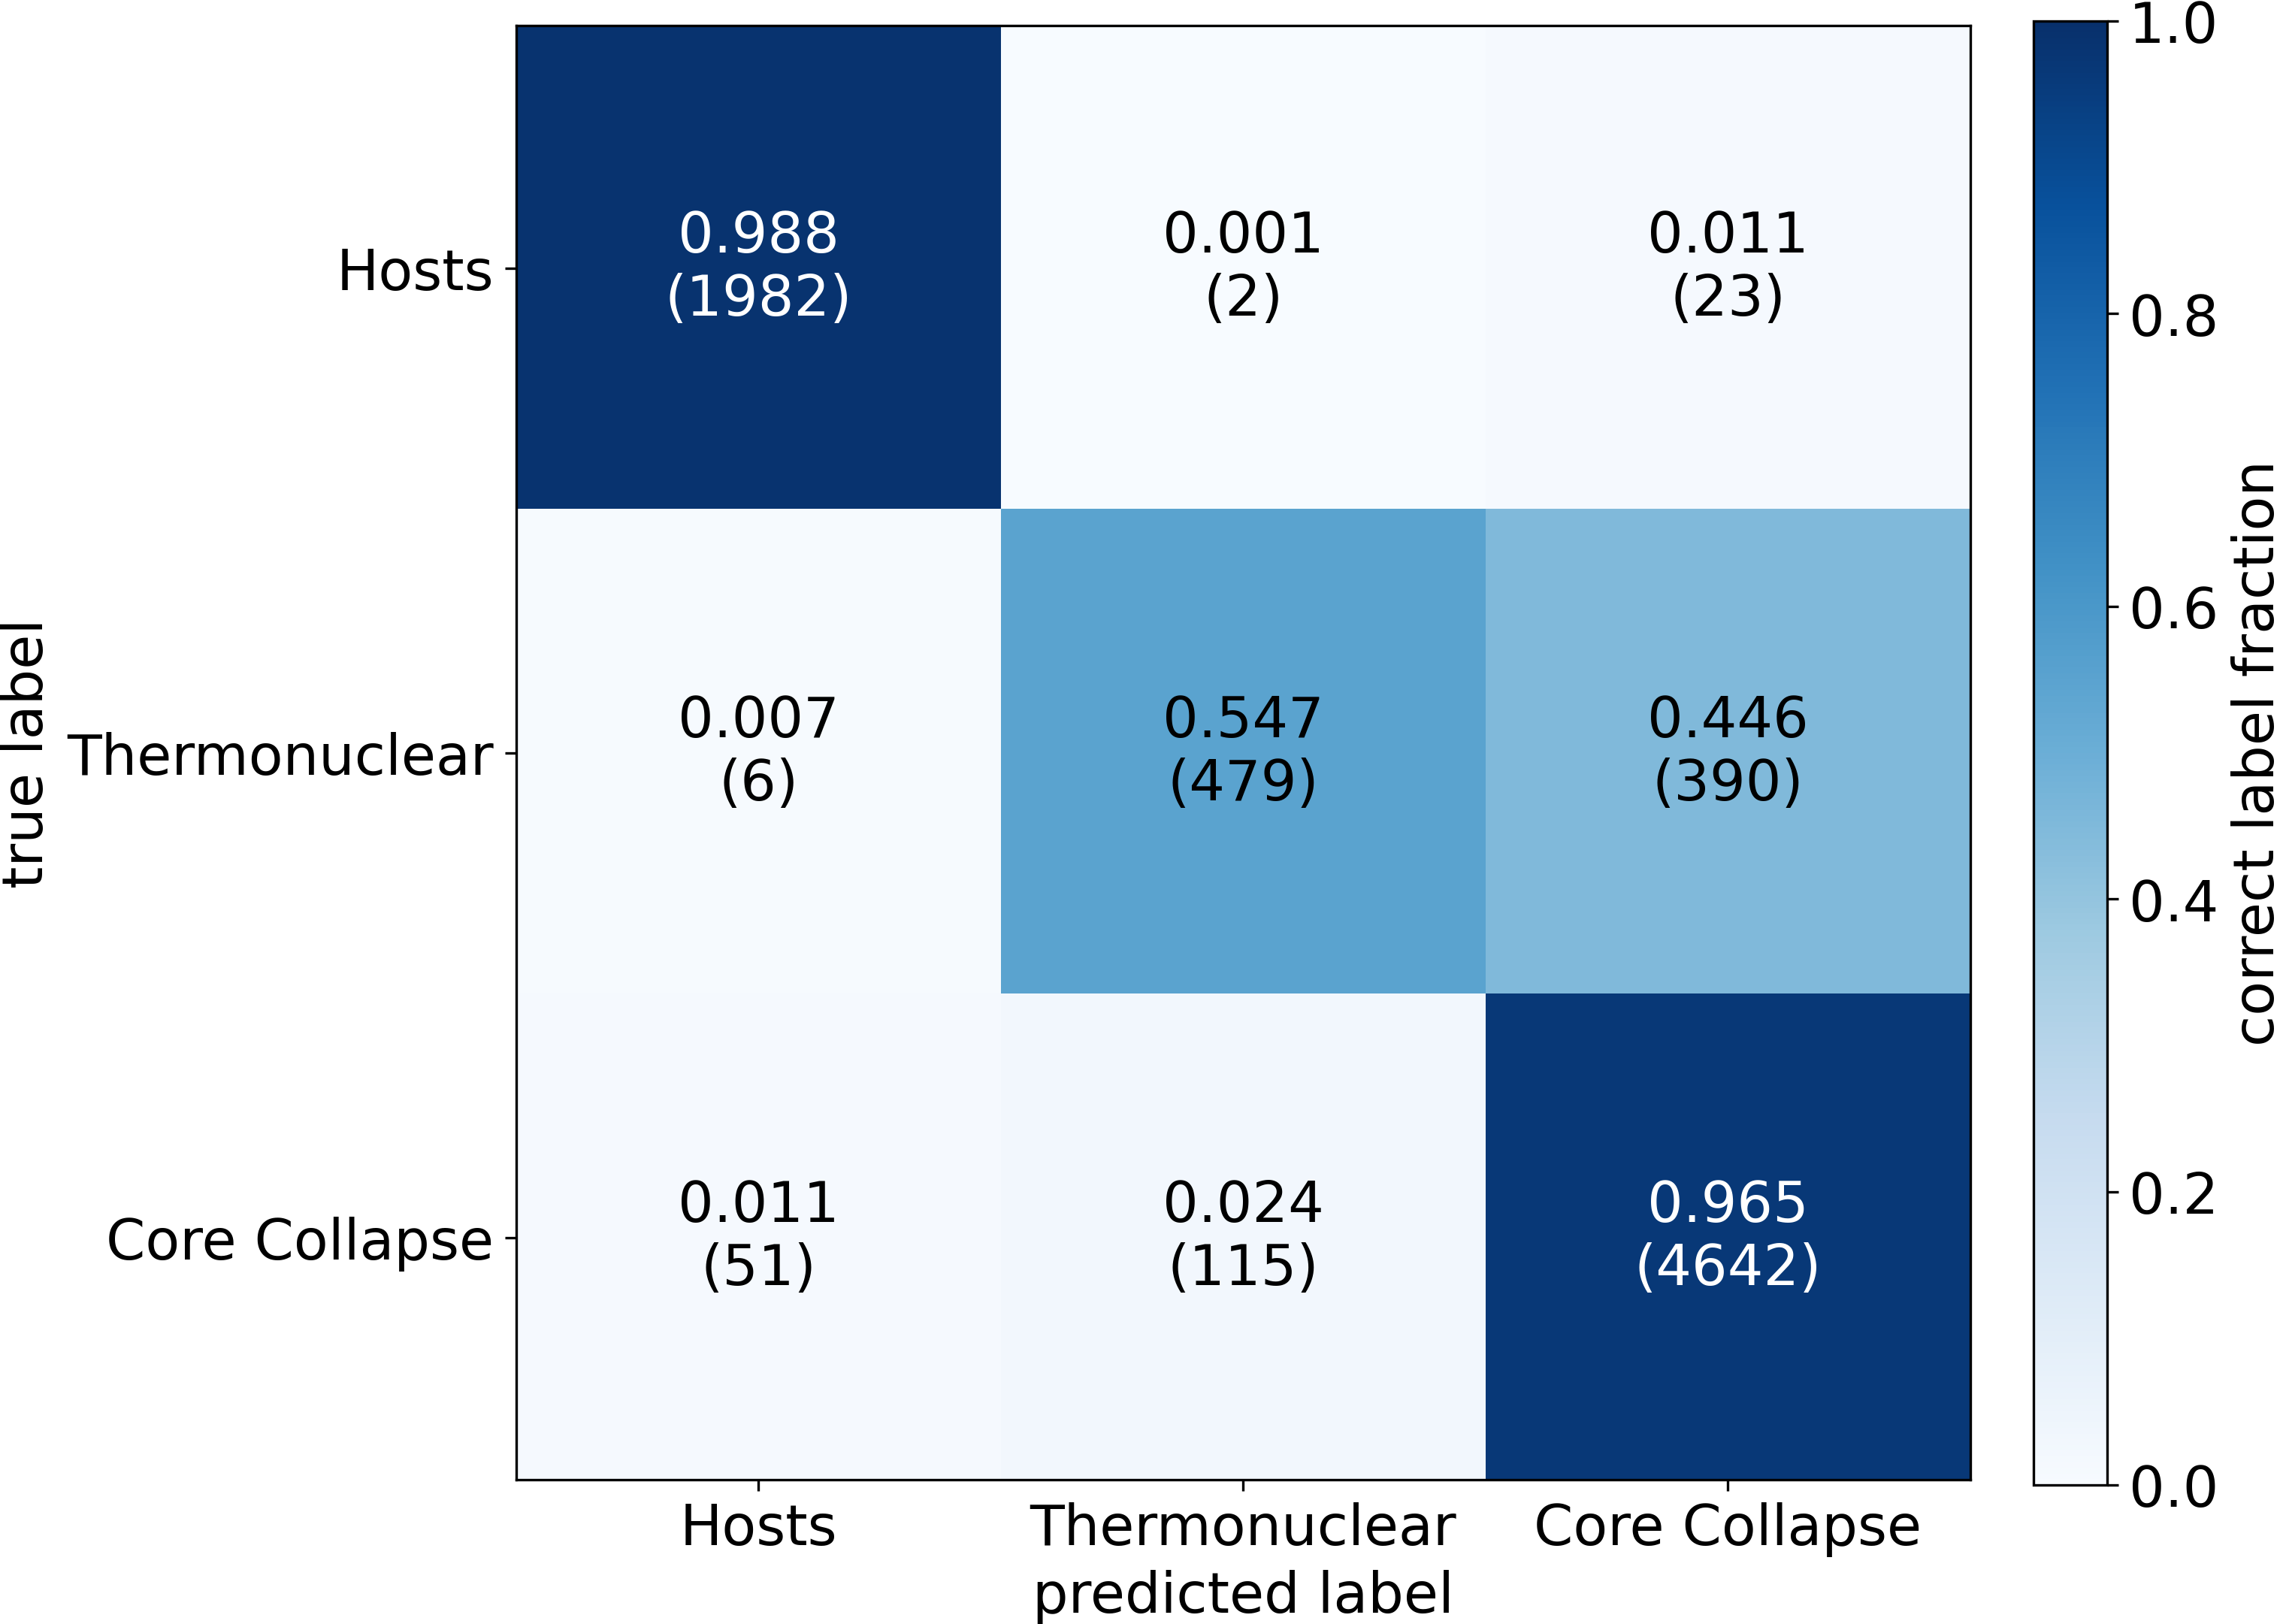
\includegraphics[height=4.1cm]{figures/v2_applications/vit_model_V2cm99_proj_e26.png}
    \caption[Spectral ViT V2 Progenitor Classifier Diagnostics]{Spectral ViT V2 
    Progenitor Classifier Diagnostics: ROC Curve (left) and Confusion Matrix (right) with a 99\% confidence
    cut\label{fig:v2_99_proj_qual}}
\end{figure}
Beyond binary classification, the Spectral ViT V2 shows the capability to differentiate between 
thermonuclear SNe (Type Ia) and core collapse SNe (Types Ib,c, and Type II). With a 99\% confidence 
cut, the classifier is able to retain 60\% of the original sample, shown in Figure~\ref{fig:v2_99_proj_qual}. 
Despite the great success in differentiating the core collapse and non-SNe spectra, there is some discrepancy 
between the two SNe categories. This, however, still results in an average precision of 86.5\% which is slightly
below the Spectral ViT V1 classifier on all subtypes, while recovering much of the original sample. 
\begin{figure}[hb!]
    \centering
    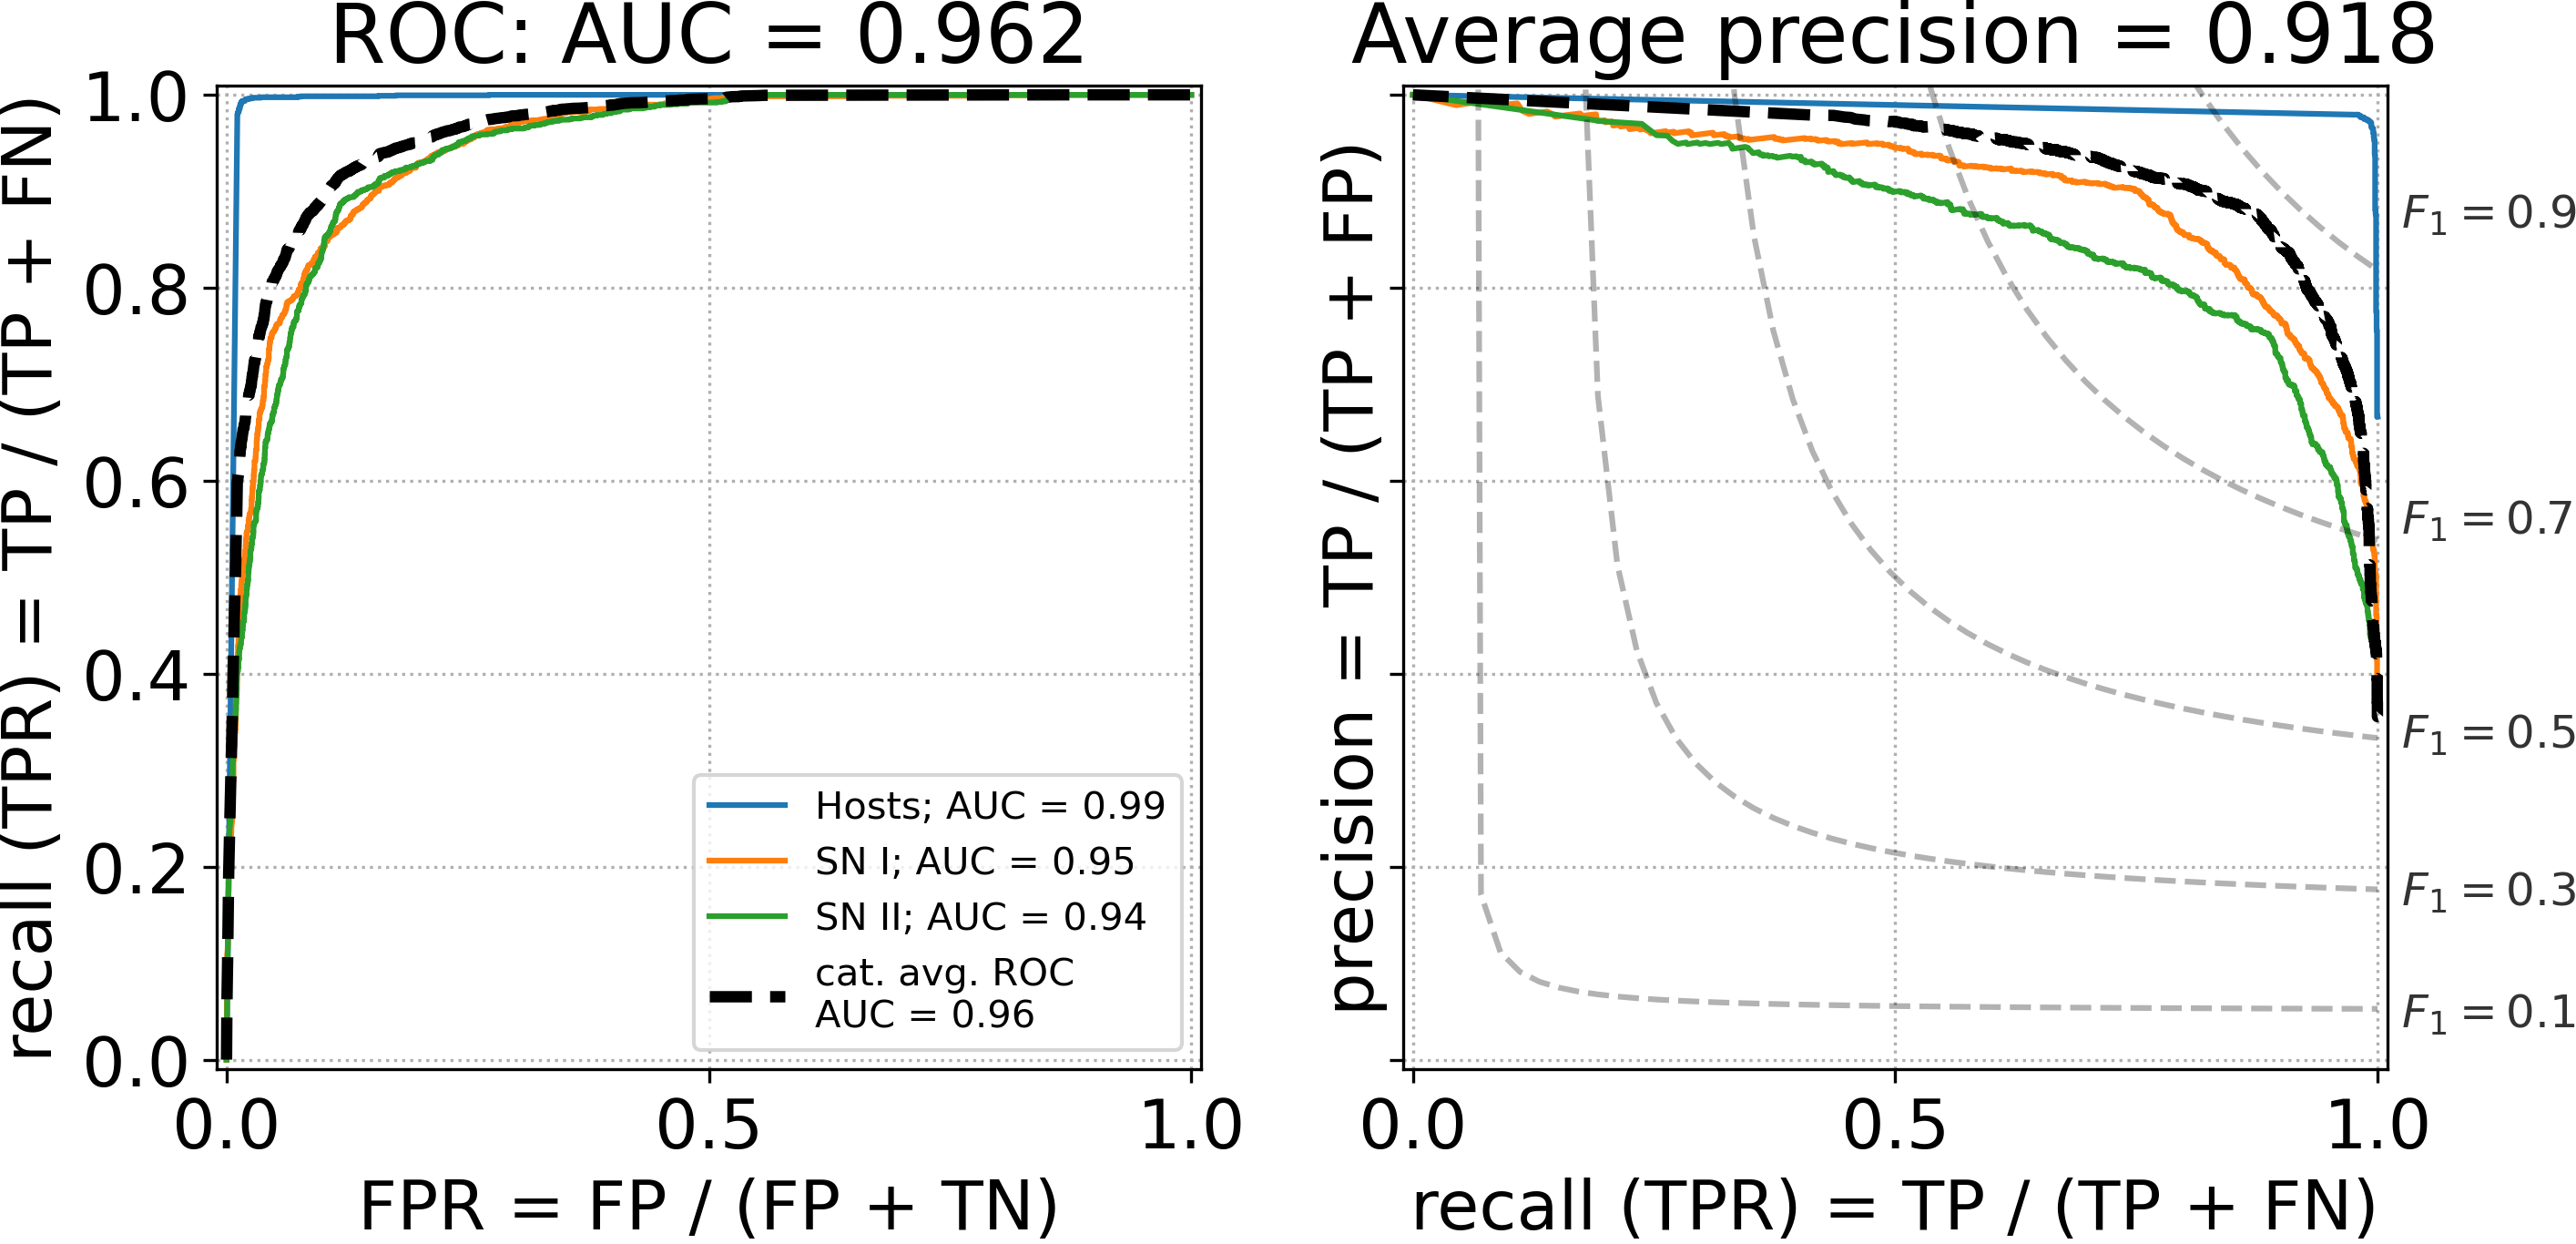
\includegraphics[height=4.1cm]{figures/v2_applications/vit_model_V2roc99_type_e26.png}
    \quad
    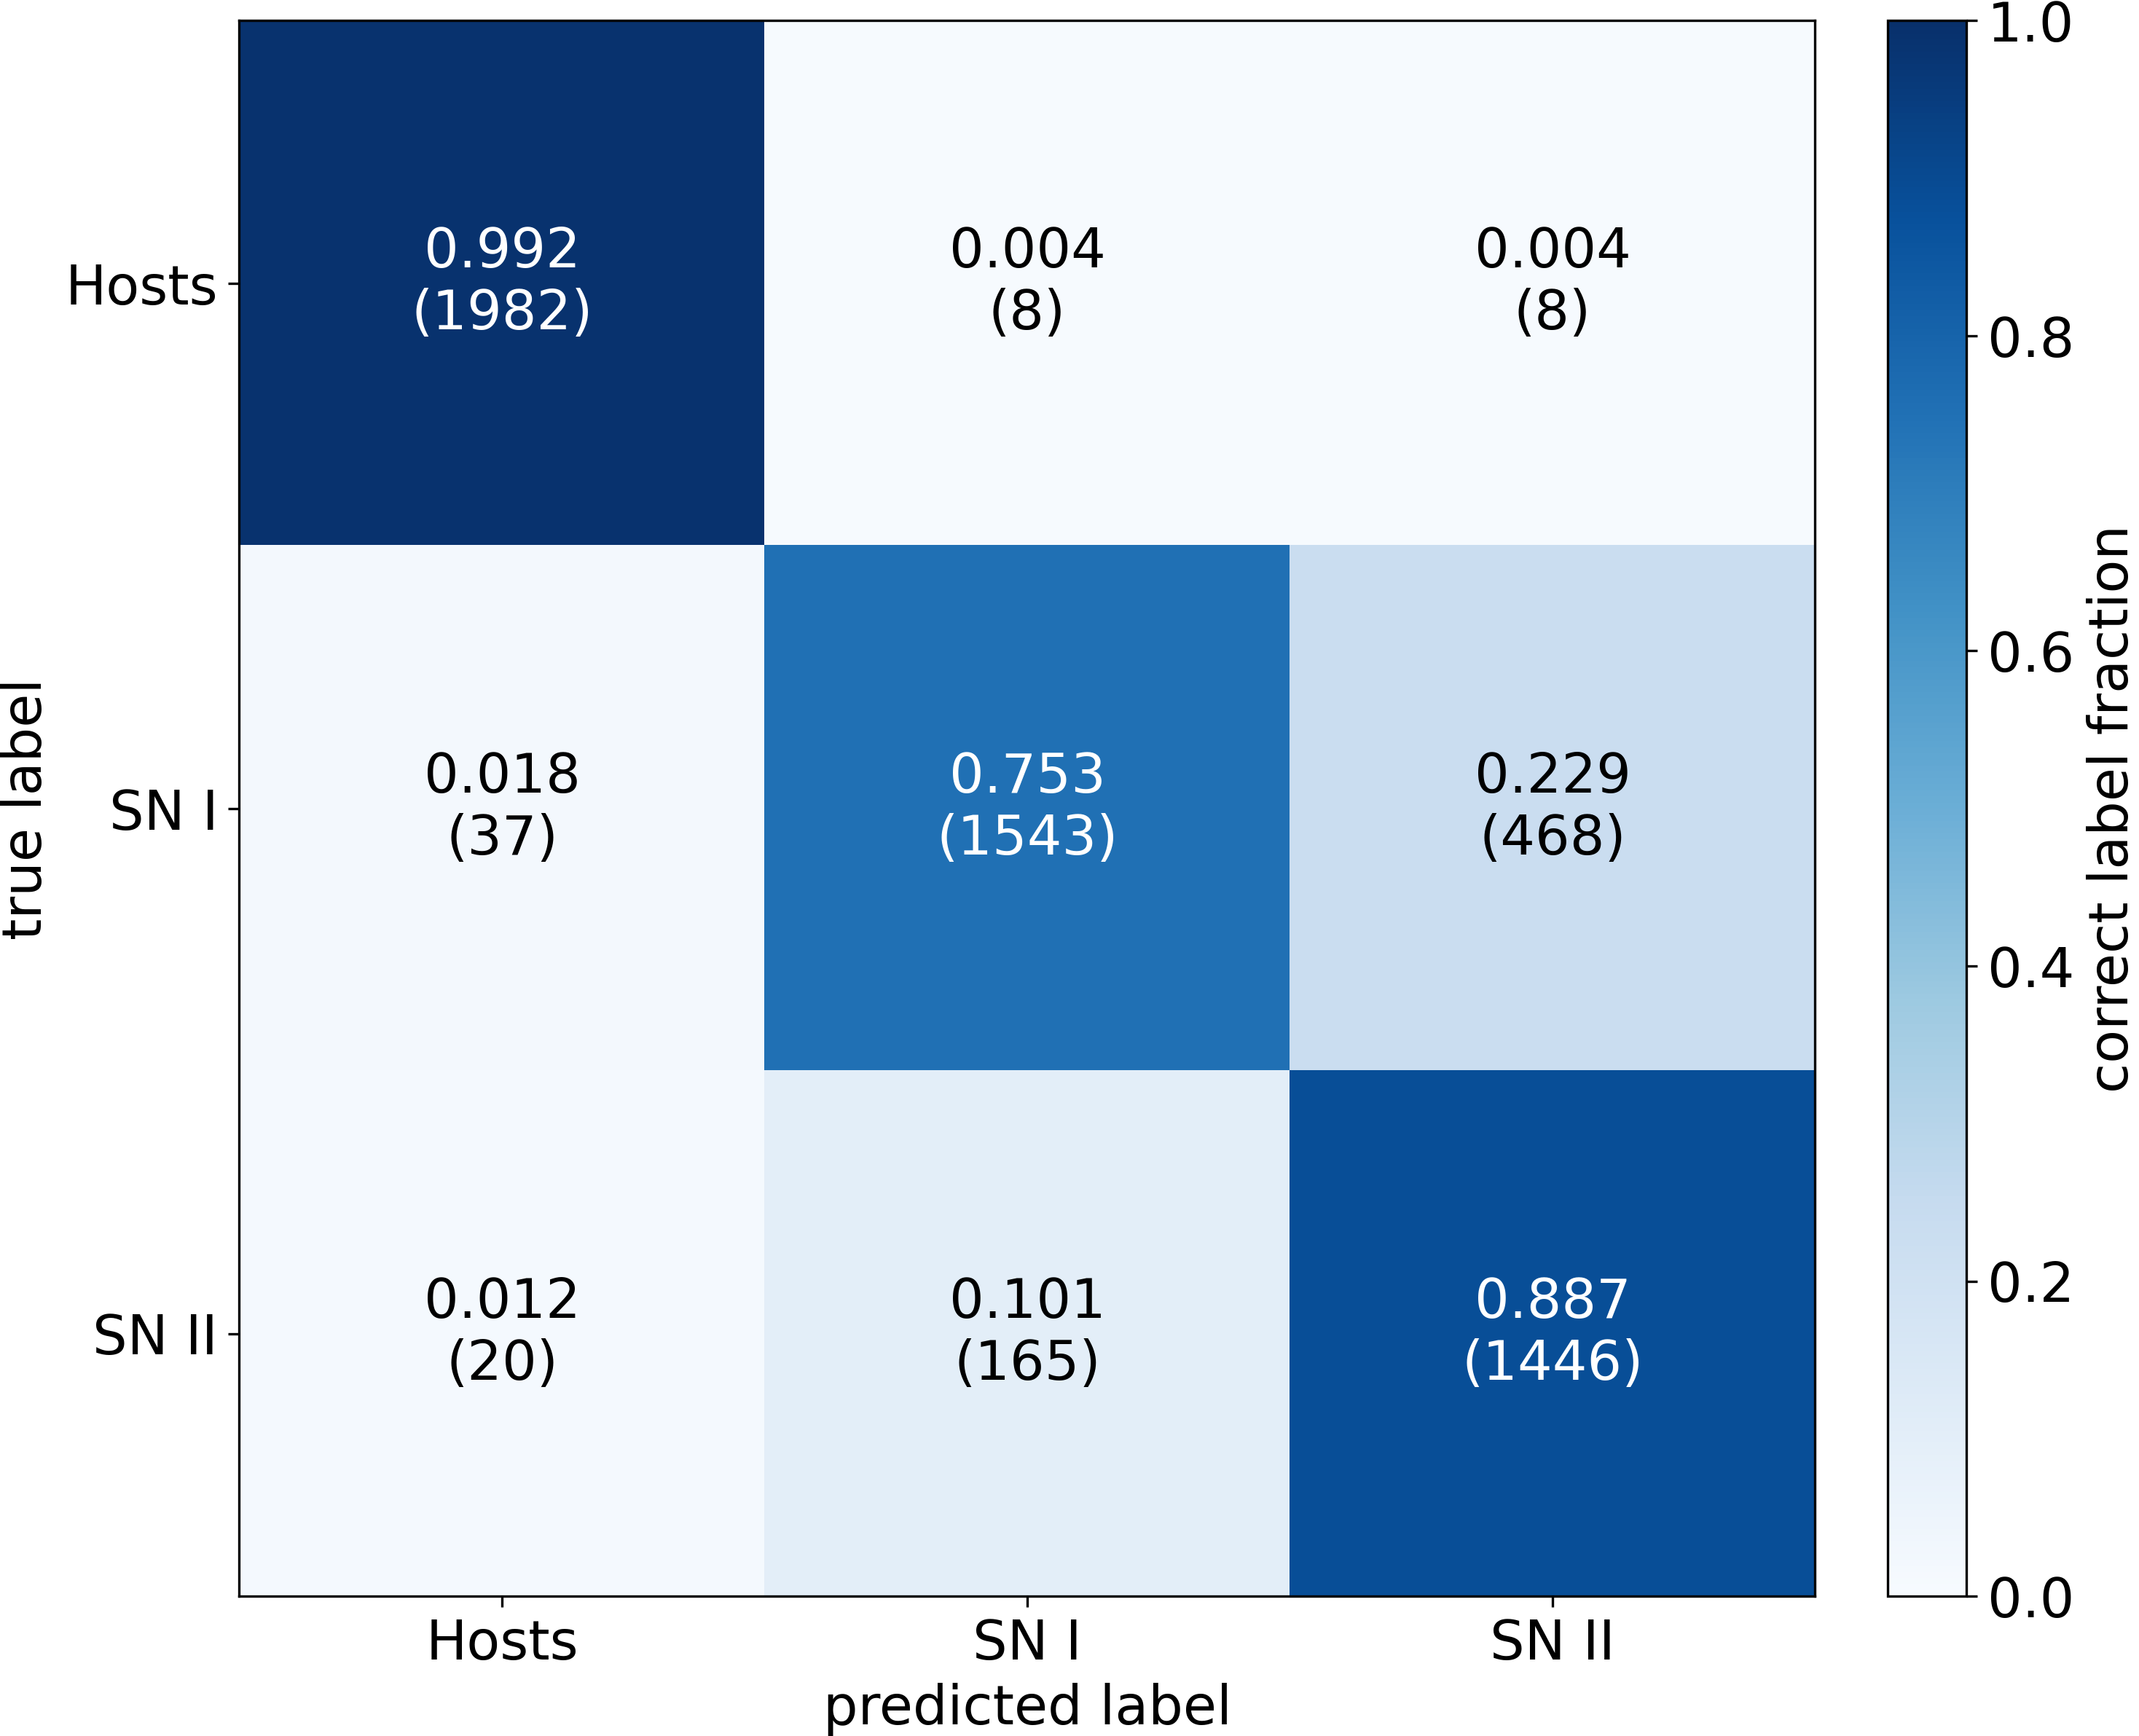
\includegraphics[height=4.1cm]{figures/v2_applications/vit_model_V2cm99_type_e26.png}
    \caption[Spectral ViT V2 Type Classifier Diagnostics]{Spectral ViT V2 
    Type Classifier Diagnostics: ROC Curve (left) and Confusion Matrix (right) with a 99\% confidence
    cut\label{fig:v2_99_type_qual}}
\end{figure}
Another classification scheme using three final classes would be to seperate the sample into the 2 main 
classifications: Type I vs Type II. Figure~\ref{fig:v2_99_type_qual} shows the 99\% cut on this classifications, 
yielding 44\% of the original sample classified at an average precision of 91.8\%. Therefore, the Spectral ViT V2
has many classification applications past just a binary classifier, regardless of its inability to produce precise 
classification of SNe subtypes.



% \begin{figure}[h]
%     \centering
%     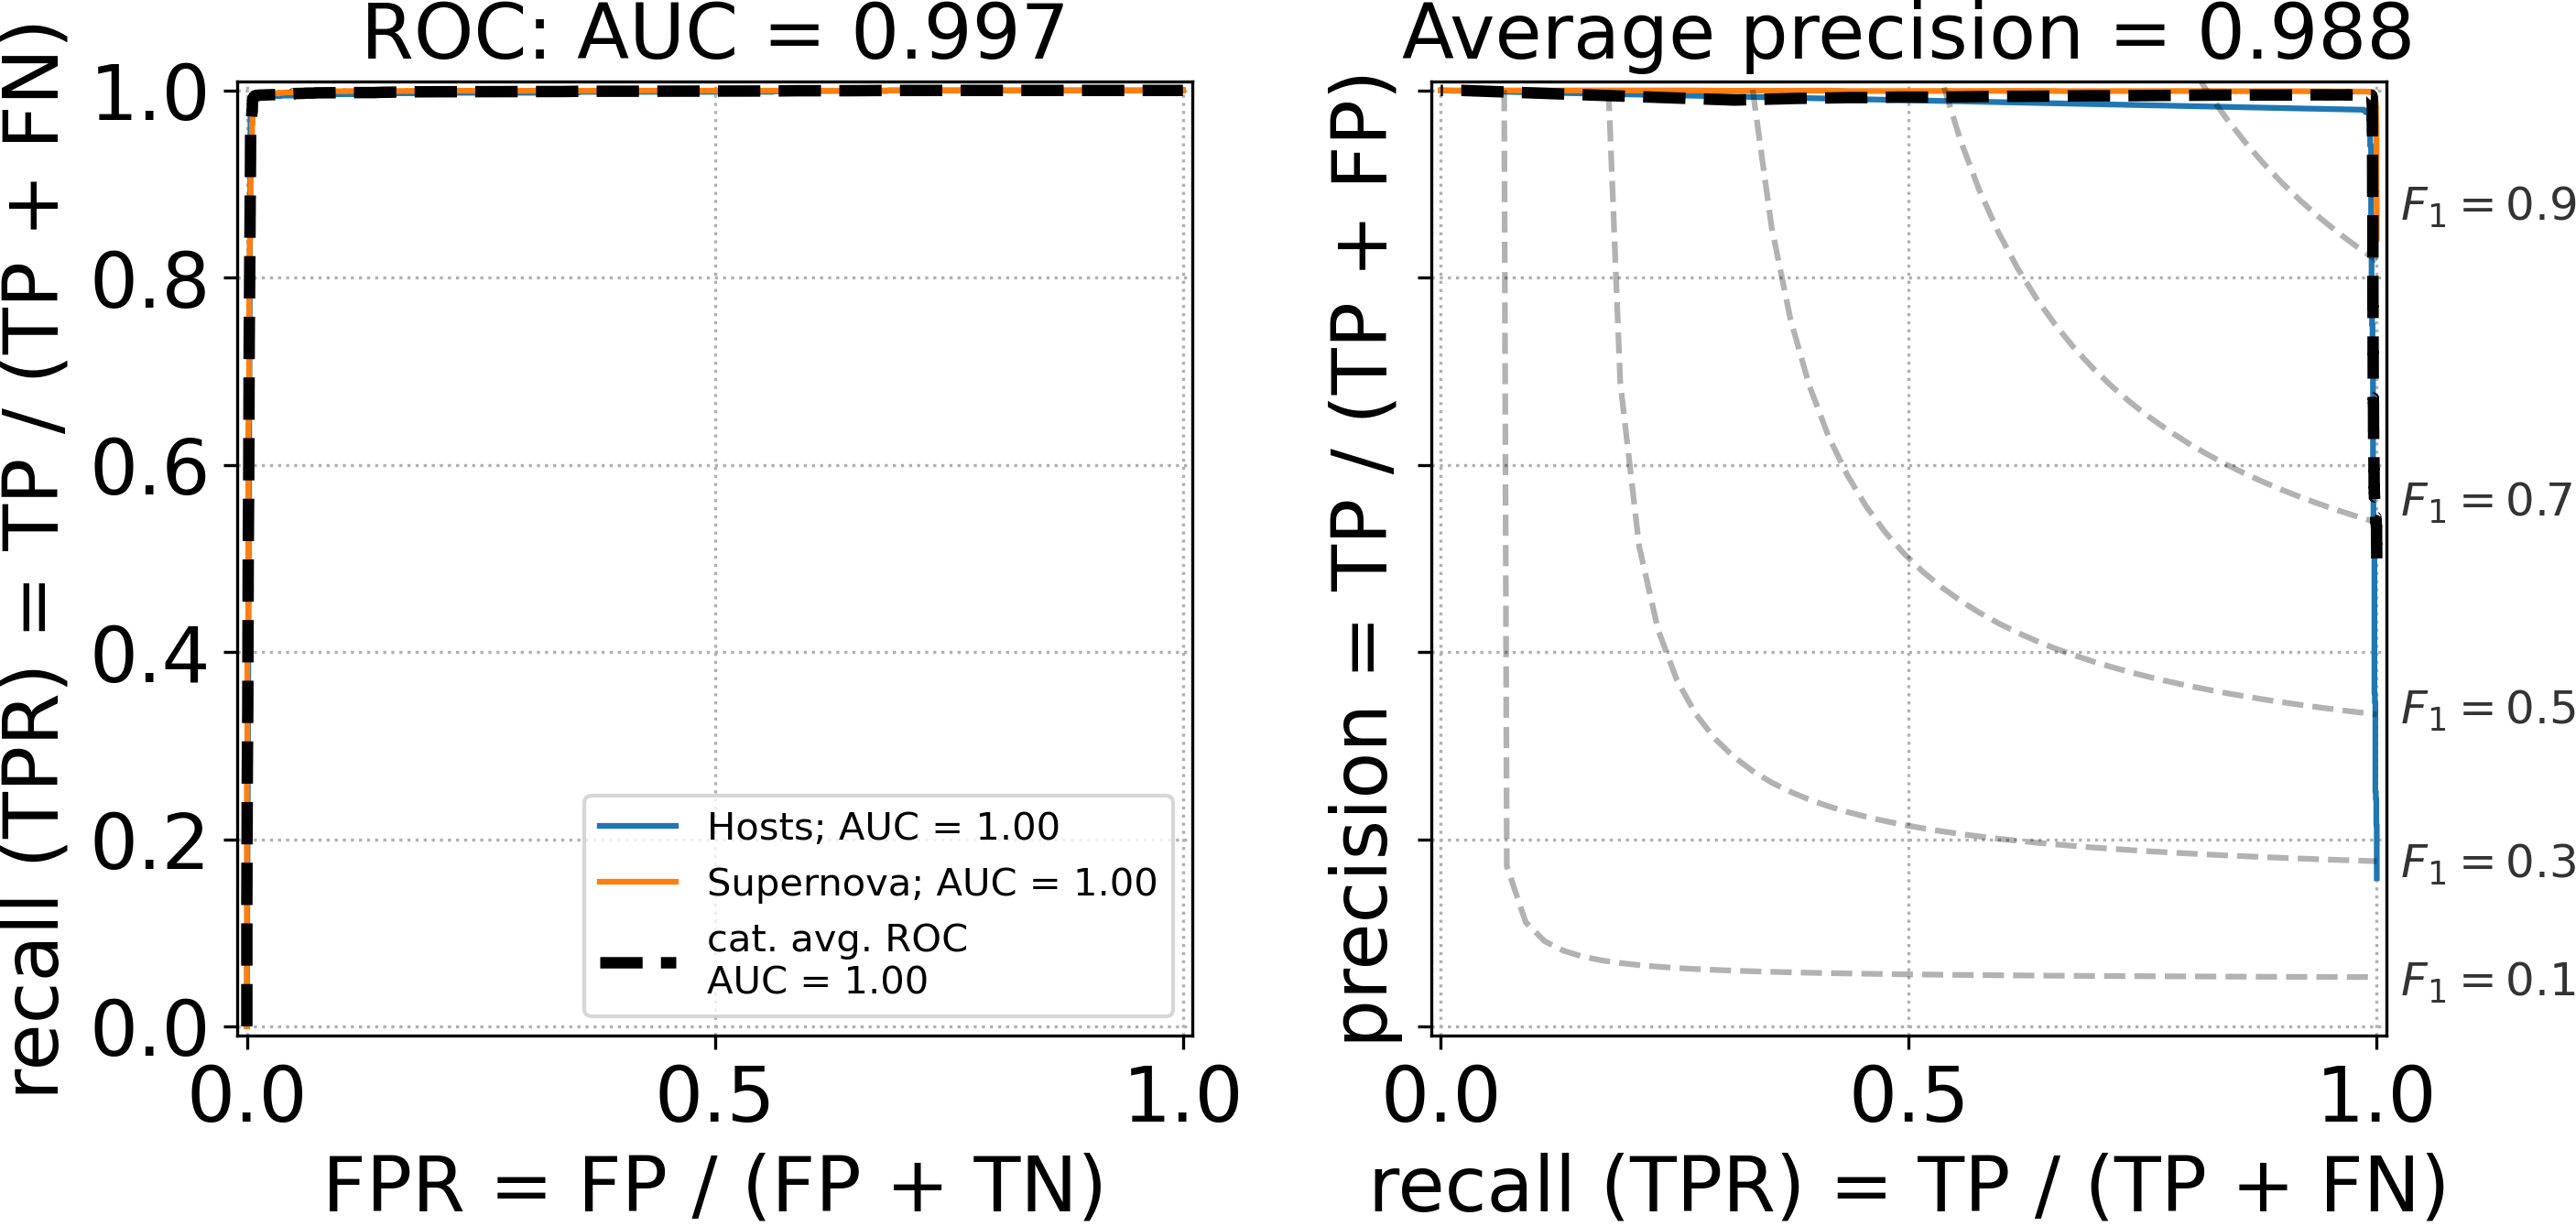
\includegraphics[height=4.2cm]{figures/v2_real/vit_model_V2roc9999_binary_e26.png}
%     \quad
%     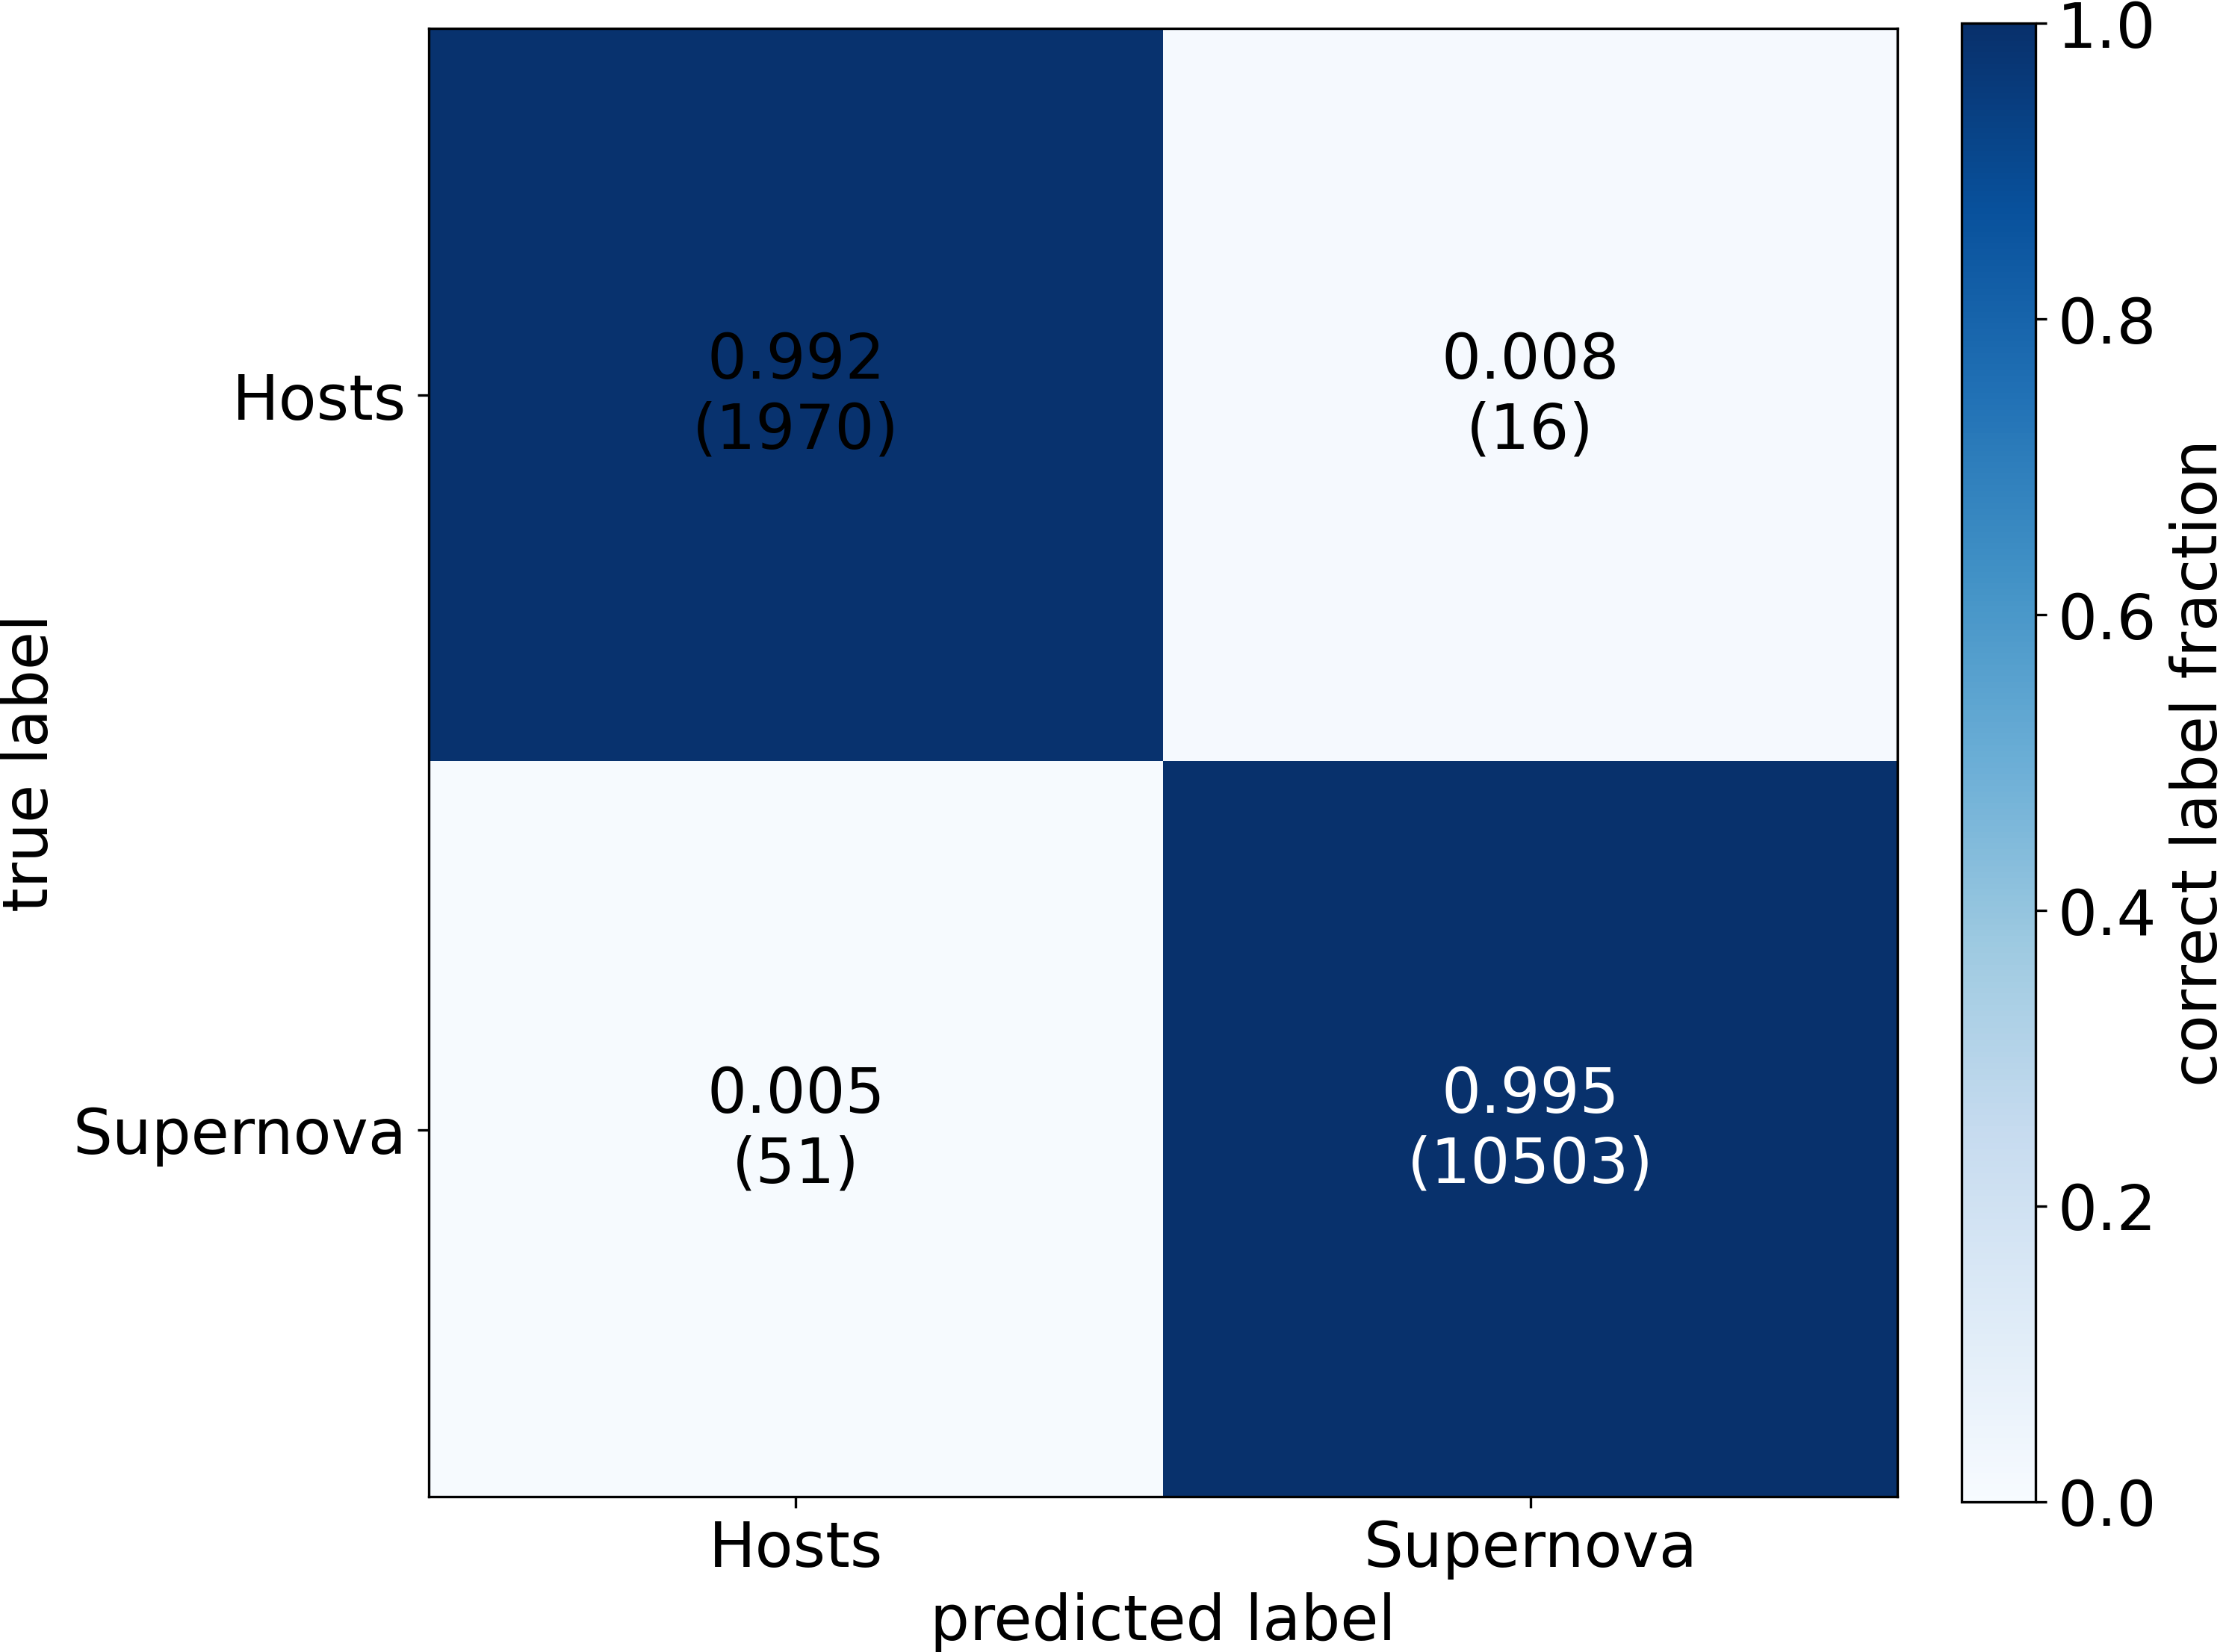
\includegraphics[height=4.2cm]{figures/v2_real/vit_model_V2cm9999_binary_e26.png}
%     \caption{Spectral ViT V2 Binary Diagnostics: ROC Curve (left) and Confusion Matrix (right) with a 99.99\% confidence
%     cut \label{fig:v2_binary_9999_qual}}
% \end{figure}

